%\documentclass[review]{elsarticle}
\documentclass[final,3p,times,twocolumn]{elsarticle}
\usepackage{amssymb}
\usepackage{amsthm}


%\usepackage[utf8]{vietnam}
\setlength{\parskip}{10pt}

\usepackage{mwe}    % loads »blindtext« and »graphicx«
\usepackage{subfig}
\usepackage{float}
\usepackage{subfloat}

\usepackage{mathtools}

\usepackage{graphics}
\graphicspath{{Figures/}}

% %Packages used to make a confusion matrix
\usepackage{tabularx}
\usepackage{colortbl}
\usepackage{hhline}

\usepackage{lineno,hyperref}
\modulolinenumbers[5]

\journal{Journal of NeuroComputing Templates}

\captionsetup[subfigure]{subrefformat=simple,labelformat=simple,listofformat=subsimple}
\renewcommand\thesubfigure{(\alph{subfigure})}

\usepackage{natbib}
% \biboptions{sort&compress}
%%%%%%%%%%%%%%%%%%%%%%%
%% Elsevier bibliography styles
%%%%%%%%%%%%%%%%%%%%%%%
%% To change the style, put a % in front of the second line of the current style and
%% remove the % from the second line of the style you would like to use.
%%%%%%%%%%%%%%%%%%%%%%%

%% Numbered
%\bibliographystyle{model1-num-names}

%% Numbered without titles
%\bibliographystyle{model1a-num-names}

%% Harvard
%\bibliographystyle{model2-names.bst}\biboptions{authoryear}

%% Vancouver numbered
%\usepackage{numcompress}\bibliographystyle{model3-num-names}

%% Vancouver name/year
%\usepackage{numcompress}\bibliographystyle{model4-names}\biboptions{authoryear}

%% APA style
%\bibliographystyle{model5-names}\biboptions{authoryear}

%% AMA style
%\usepackage{numcompress}\bibliographystyle{model6-num-names}

%% `Elsevier LaTeX' style
\bibliographystyle{elsarticle-num}
%%%%%%%%%%%%%%%%%%%%%%%

\begin{document}

\begin{frontmatter}

\title{DTOP: Dense Trajectories on Planes for Action Recognition from Depth Sequences}

%% Group authors per affiliation:
%\author{Chien-Quang LE}
%\address{The Graduate University for Advanced Studies}
%
%\author{Thanh-Duc NGO}
%\address{Adress 1}
%
%\author{Duy-Dinh LE}
%\address{National Institute of Informatics, The Graduate University for Advanced Studies}
%
%\author{Duc-Anh DUONG}
%\address{Adress 2}
%
%\author{Shin'ichi SATOH}
%\address{National Institute of Informatics, The University of Tokyo}

\author{Author name}
\address{Work address}

\author{Author name}
\address{Work address}

\begin{abstract}
Dense trajectory-based approaches on 2D video have been demonstrated state-of-the-art at action recognition since it can capture most discriminative motions.
However, there are not many studies related to exploiting the discriminative motions in depth video.
In this work, we extend the approach on depth video and show its effectiveness for action recognition.
We extract dense trajectories from 2D videos transformed from depth video and apply trajectory-aligned descriptors to calculate motion features.
To obtain the 2D transformed videos, we build views, which can capture the discriminative motions similar to observing actions from different directions.
We evaluate this approach on framework of action recognition using the benchmark MSR Action 3D, MSR Gesture 3D and 3D Action Pairs datasets.
Evaluation results show that our proposed approach is effective for action recognition on depth video and outperforms the state-of-the-art approaches.
\end{abstract}

\begin{keyword}
\texttt{Motion pattern, dense trajectories, action recognition, depth map, projection}
%\MSC[2010] 00-01\sep  99-00
\end{keyword}

\end{frontmatter}

\linenumbers

\section{Introduction}

%\paragraph{Background and Challenges}
Action recognition in videos has been one of the active research fields in computer vision \cite{pirsiavash2012detecting, poppe2010survey} due to its wide applications in areas like surveillance, video retrieval, human-computer interaction and smart environments.
Due to the diversity and complexity of actions, as well as complicated environment (e.g background clutter and illumination variation), action recognition is still a challenging problem.
Recent approaches can be divided into three major categories: silhouette-based \cite{blank2005actions, ke2007event, vitaladevuni2008action, yilmaz2005actions}, salient point-based \cite{laptev2005space, dollar2005behavior, laptev2008learning, bregonzio2009recognising, klaser2008aspatiotemporal, willems2008efficient} and trajectory-based \cite{matikainen2009trajectons, messing2009activity, sun2009hierarchical}.
All approaches, basically, try to capture motion information that appears in videos, since motion is crucial information for presenting actions.
Based on recent works \cite{phan2014multimedia, oneata2012axes, natarajan2012bbn}, exploiting discriminative motion patterns has been demonstrated successful at action recognition.
%Based on work of H.Wang et al. \cite{wang2011densetraj}, dense trajectory-based approach has been demonstrated that it is the state-of-the-art approach for action recognition \cite{phan2014multimedia, oneata2012axes, natarajan2012bbn}.
%Recently, the dense trajectory-based motion feature proposed by \cite{wang2011densetraj} has achieved the state-of-the-art performances on multimedia event detection (MED) systems, such as, segment-based system \cite{phan2014multimedia} on TRECVID MED 2010, 2011, or AXES \cite{oneata2012axes}, and BBNVISER \cite{natarajan2012bbn} on TRECVID MED 2012.

%\paragraph{Existing approaches and drawbacks}
With relative works, most studies mainly investigate on video sequences captured by traditional 2D cameras.
Although, there are many improvements on the approach for action recognition in domain of 2D videos \cite{jain2013better, wang2013action}, the mentioned challenges are still difficult to handle.
With the development of new RGB-D cameras, e.g. Kinect camera, capturing color images as well as depth maps has become feasible in real time.
The depth maps can enrich information for cues, such as body shape and motion information.
In addition, depth information is less sensitive to the challenges RGB information usually deals with.
Due to these advantages, recent research trend concentrates on exploiting depth maps for action recognition \cite{li2010action, wang2012mining, vieira2012stop, yang2012eigenjoints, yang2012recognizing, wang2012robust, xia2013spatio, oreifej2013hon4d, luo2013group}.
However, with our best knowledge, none success with combining discriminative motion pattern-based approach, the state-of-the-art on 2D video, on depth video.
In this paper, we investigate to exploit the approach on depth video.

\begin{figure*}[t]
	\centering
	\resizebox{\textwidth}{!}{
		\begin{tabular}{ccc}
	       \subfloat[Action \textit{Hammer}]{
		         		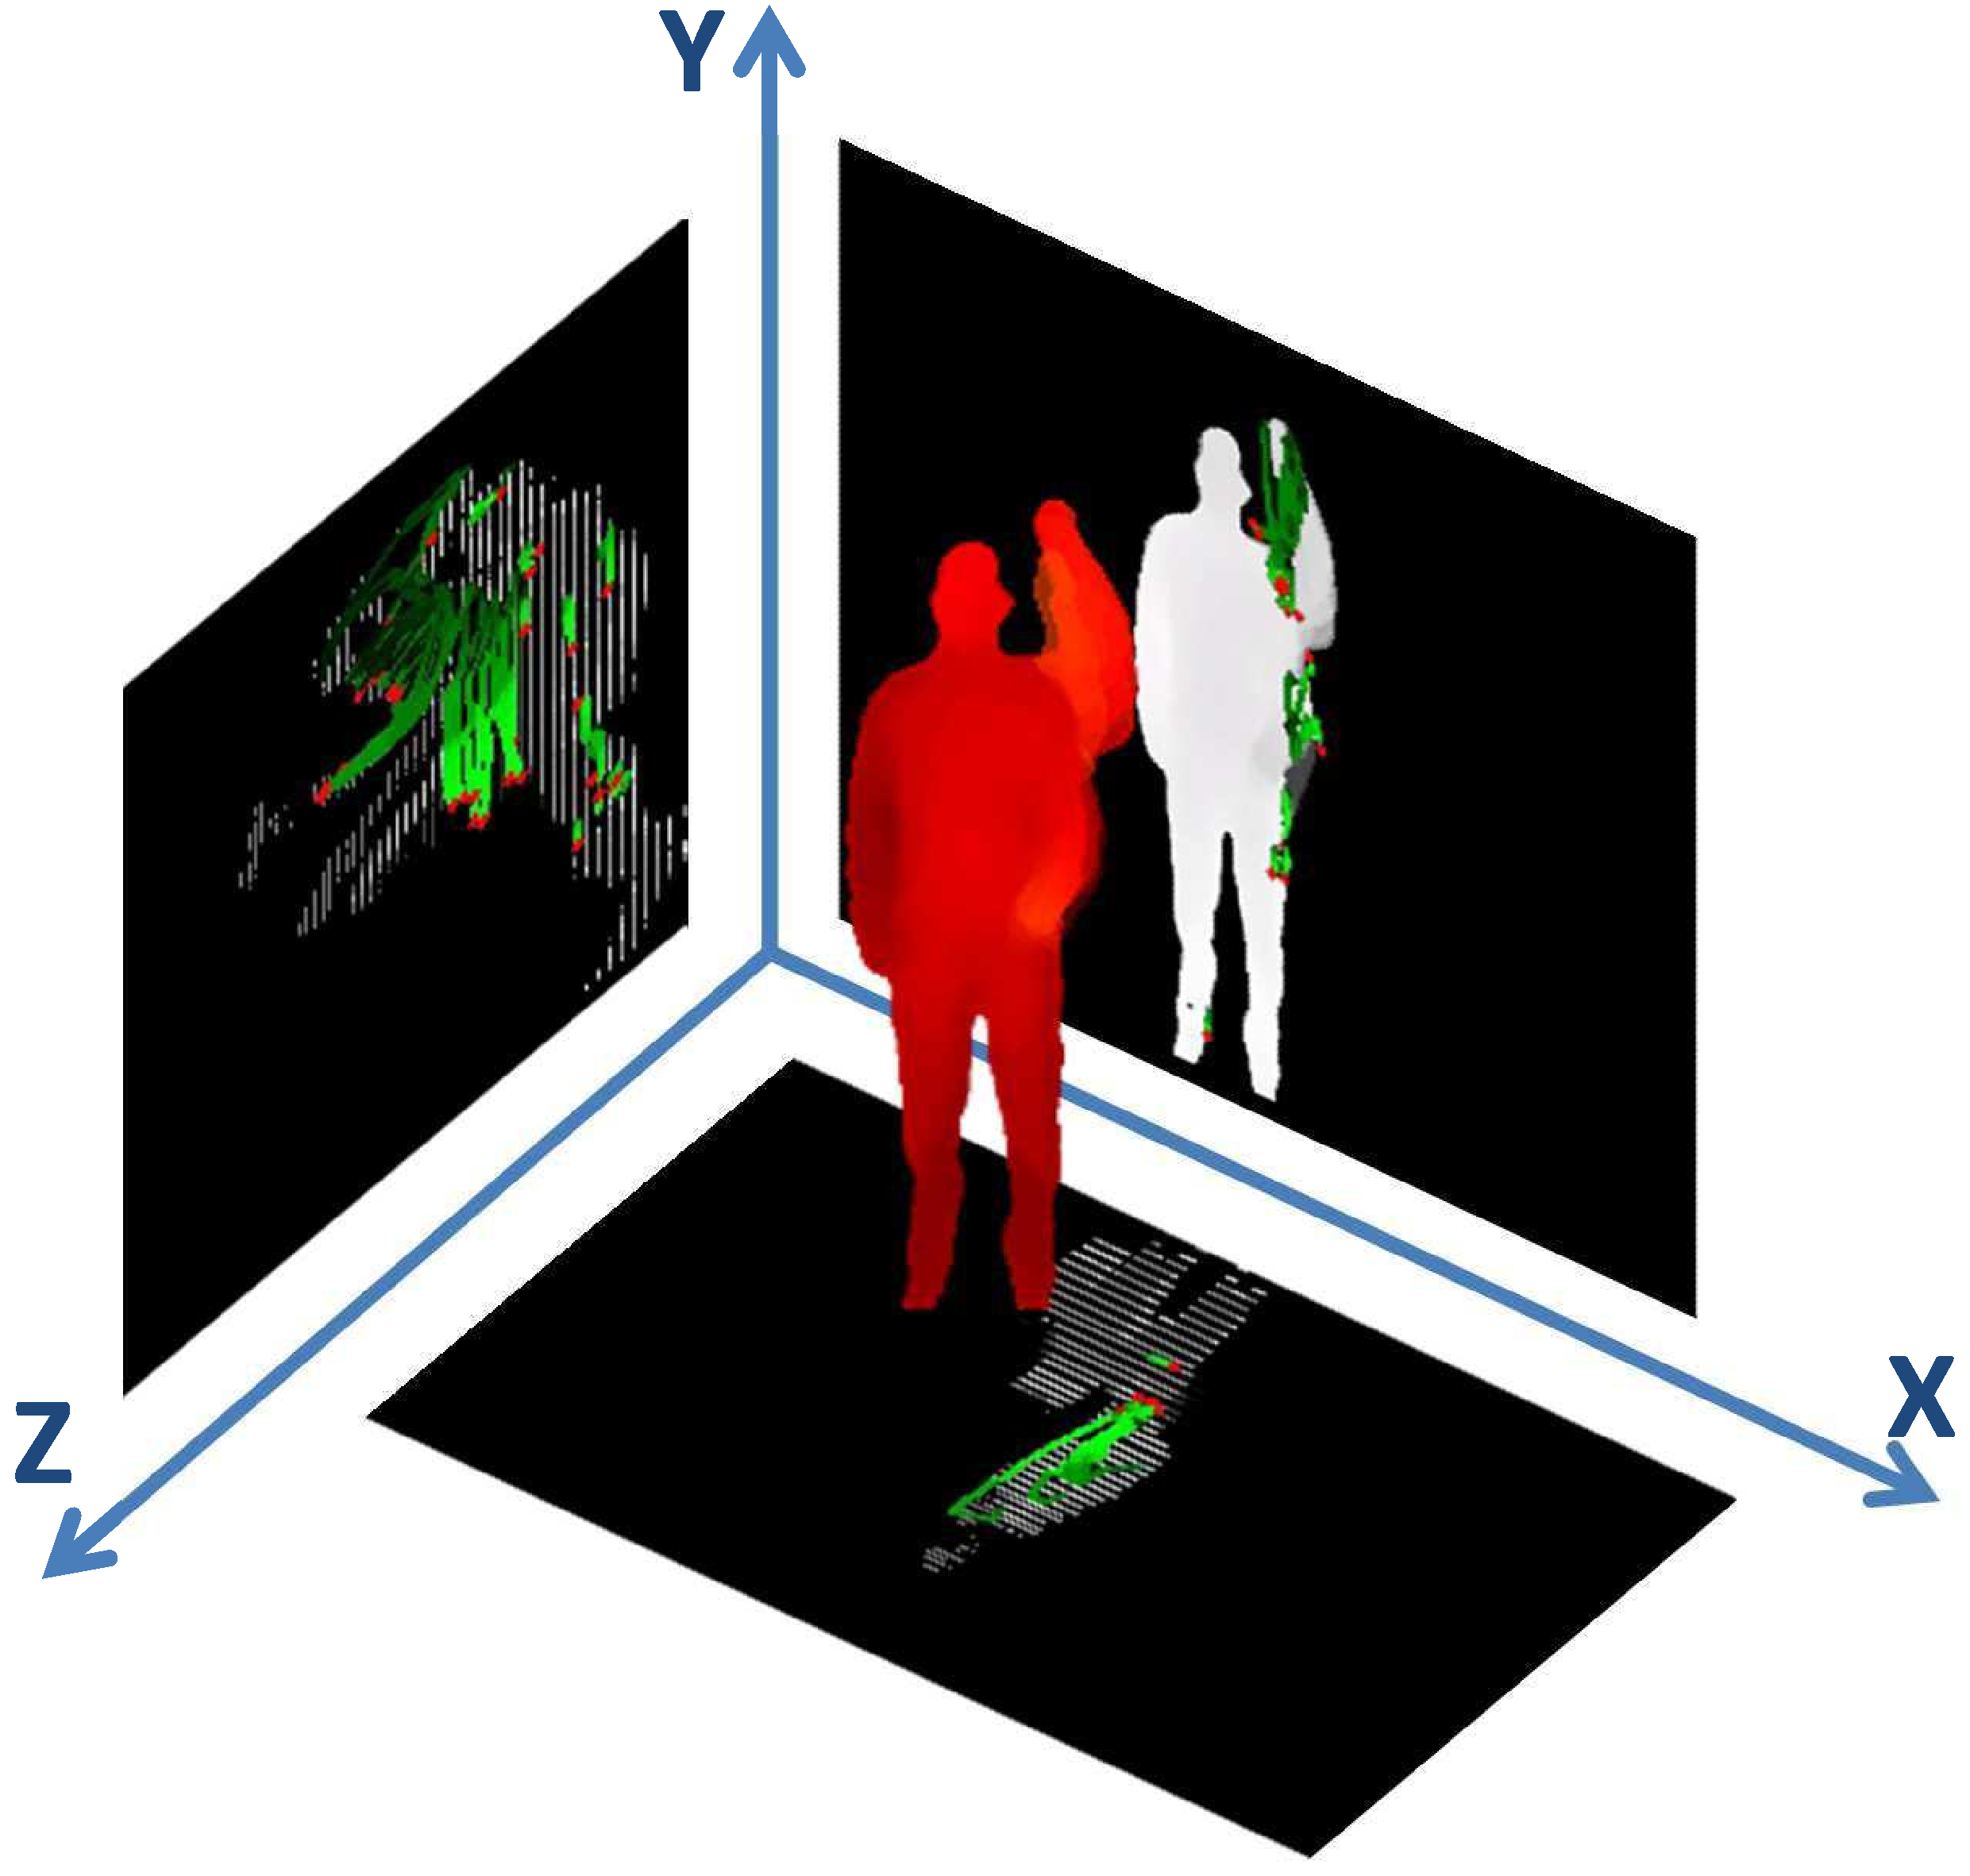
\includegraphics[width=0.4\textwidth]{Figures/Figure_Hammer3D.pdf}
		         		\label{subfig_Hammer3D}
		         	} &
   		   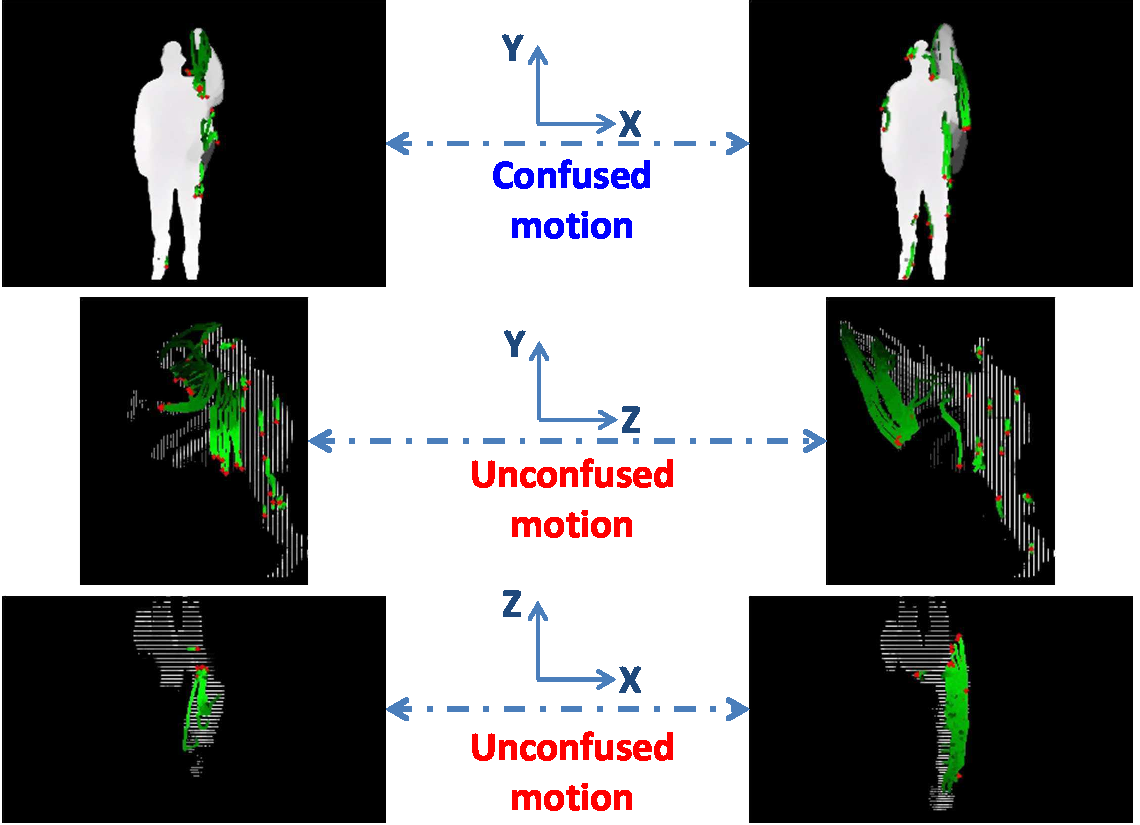
\includegraphics[width=0.4\textwidth]{Figures/Figure_ComparisonPlanes.pdf} &
	       \subfloat[Action \textit{Forward Punch}]{
		         		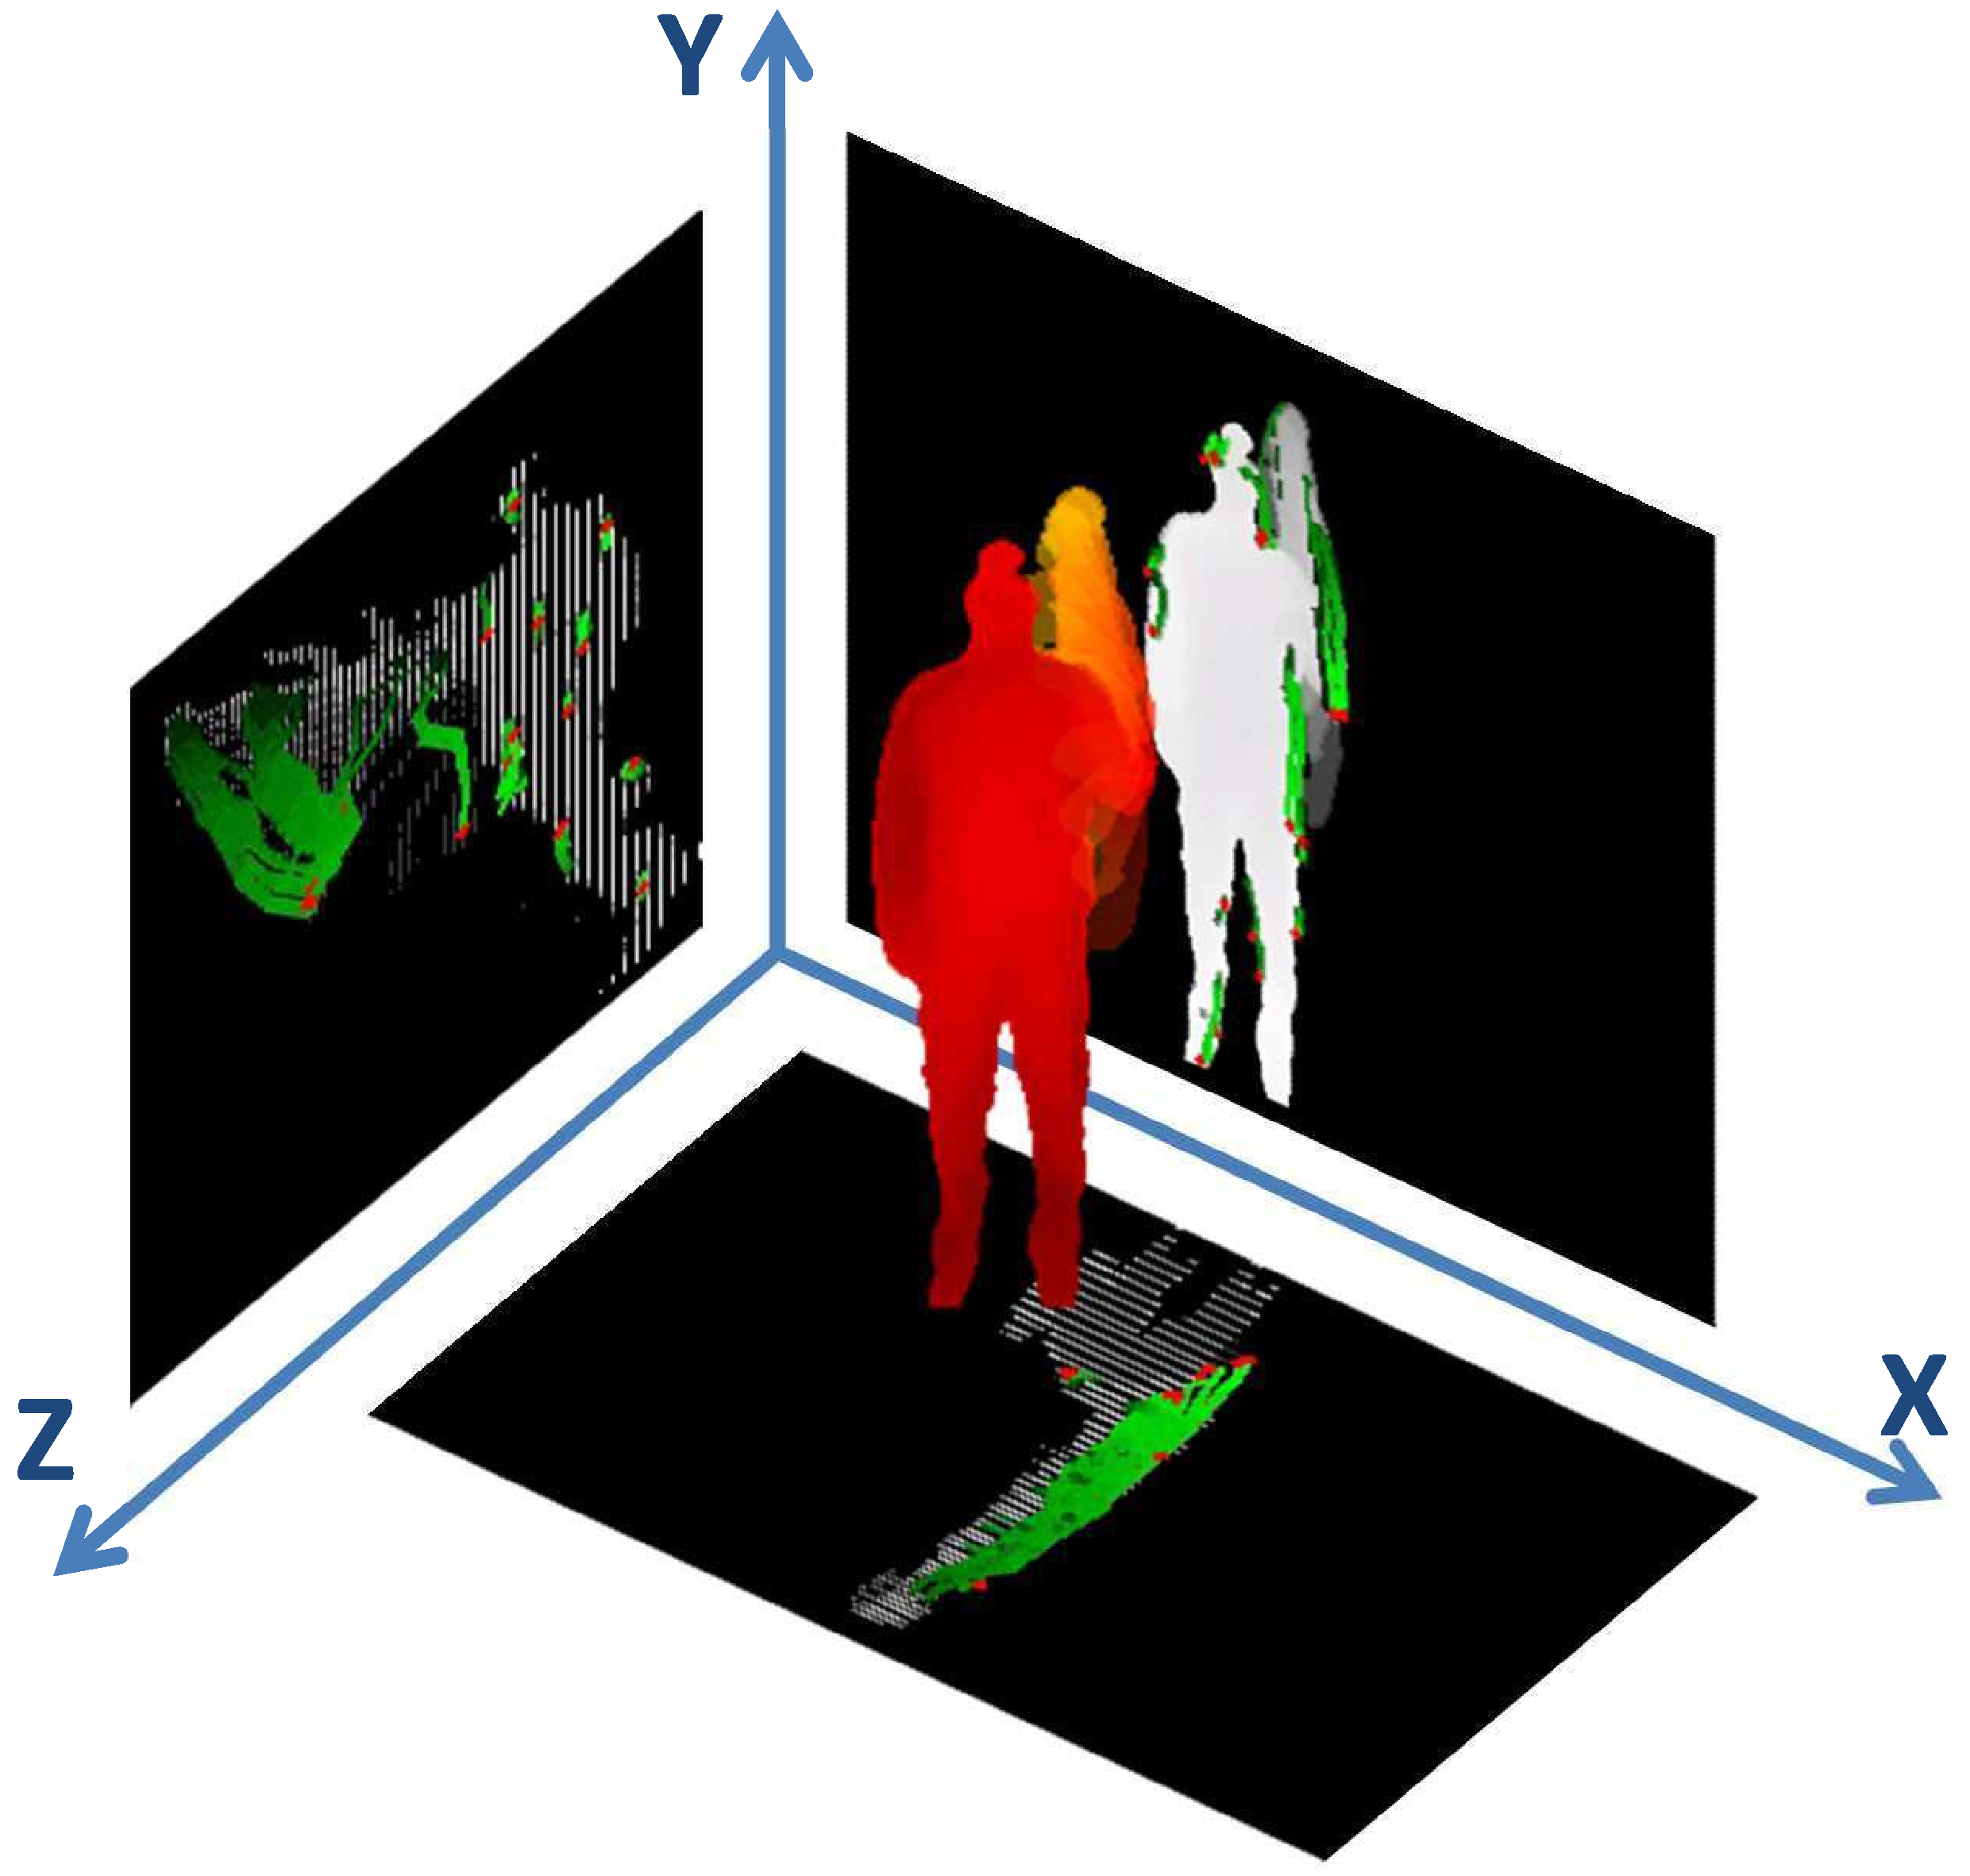
\includegraphics[width=0.4\textwidth]{Figures/Figure_ForwardPunch3D.pdf}
		         		\label{subfig_ForwardPunch3D}
		         	} \\
		\end{tabular}  
		
	}
	\caption{Illustration of our dense trajectory-based approach. The original sequence of depth maps is projected onto three planes, corresponding to three views: \textit{front}, \textit{side} and \textit{top}, to form 2D videos. After that, the dense trajectory motion features are calculated for each 2D video.}
		\label{Figure_ProposedMethod}
\end{figure*}

%\paragraph{Proposal, Idea and Steps}
The key idea of the approach is to capture discriminative trajectories in video.
Therefore, in order to effectively exploit this approach on depth video, it is necessary to extract the trajectories from depth video.
To do that, a straightforward method is to consider depth value as intensity value and adapts extracting dense trajectories on the 2D transformed video.
Unfortunately, the method will lead to inherent cases of the trajectory-based approaches, it is confused to identify actions contain similar motions.
For example, \textit{forward punch} and \textit{hammer} may be confused actions, if we view them from front, since they contain similar movements respectively: ``lift arm up'' and ``stretch out''.
Obviously, it is difficult to distinguish such actions with data contains less discriminative information as depth data.
This is major reason to require additional information for effectively recognizing actions.

To deal with such cases, we consider getting more information on such actions from various directions.
Information achieved from the view directions can provide clearer cues to discriminate such actions.
To collect such information from depth video, a proposed method is to project depth maps onto view planes, see figure \ref{Figure_ProposedMethod}.
The projections are easily obtained by the mentioned advantages of depth data.
Motion features are then calculated to generate corresponding projection representations.
Finally, depth video representation is formed by fusing the projection representations.

%\paragraph{Experiments and Results}
In our experiments, we adopt dense trajectory-based approach \cite{wang2011densetraj} to exploit discriminative motion patterns since that is the state-of-the-art approach for action recognition on domain of 2D videos.
To evaluate the effectiveness of proposed method, we conduct experiments on MSR Action 3D dataset, MSR Gesture 3D dataset and 3D Action Pairs dataset.
Experimental results show that our proposed method beats the state-of-the-art methods at action recognition using depth data.
The results also present our contributions: (1) we propose an effective method to exploit trajectories in depth video, (2) we perform comprehensive experiments on the challenging benchmark dataset and indicate that our proposed method is the best when compared with the state-of-the-art depth-based methods.

%\paragraph{Paper structure}
After a brief review of the related work in Section \ref{Section_RelatedWorks}, our action recognition framework is mentioned in Section \ref{Section_Framework}. The proposed method is described in Section \ref{Section_ProposedMethod}. Section \ref{Section_Experiments} presents the experimental settings and results. In section \ref{Section_Discussion} we provide some concerned discussions. The summaries of our work are given in Section \ref{Section_Conclusions}.

\section{Related Works}
\label{Section_RelatedWorks}

In terms of action recognition in 2D video, there are three popular approaches used in several action recognition systems, including silhouette-based, salient point-based and trajectory-based.
The silhouette-based approach, as described in \cite{blank2005actions, ke2007event, vitaladevuni2008action, yilmaz2005actions}, is powerful since it encodes a great deal of information in a sequence of images.
However, it is sensitive to different viewpoints, noise and occlusions.
Besides, it depends on the accuracy of localization, background subtraction or tracking for exactly extracting region of interest.
An other approach based on salient points generates a compact video representation and accepts background clutter, occlusions and scale changes.
The effectiveness of this approach is also showed in several works \cite{laptev2005space, dollar2005behavior, laptev2008learning, bregonzio2009recognising, klaser2008aspatiotemporal, willems2008efficient}.
However, in case of recognizing complicated motions, the salient point-based approach deals with several challenges, due to the lack of relationship of salient points.
In recent studies \cite{matikainen2009trajectons, messing2009activity, sun2009hierarchical}, the trajectory-based approach captures moving patterns in video, thereby it provides additional information to recognize motions more exactly.

For depth video, most recent methods exploit depth information into two major directions. The first one is to adapt 2D techniques-based methods for depth data. The second one is to use depth value as its mean.

For the first direction, Yang.X et al. \cite{yang2012recognizing} propose the Depth Motion Maps (DMM) to accumulate global activities in depth video sequences. The DMM are generated by stacking motion energy of depth maps projected onto three orthogonal Cartesian planes. And the Histogram of Oriented Gradients (HOG) \cite{dalal2005histograms} are computed from the DMM to represent an action video. Another approach proposed by Xia.L and Aggarwal.J.K \cite{xia2013spatio} presents a filtering method to extract spatio-temporal interest points from depth videos (DSTIPs). In this approach, they extend a work of Dollar et al. \cite{dollar2005behavior} to adapt for depth data. Firstly, 2D and 1D filters (e.g. Gaussian and Gabor filters) are applied respectively on to the spatial dimensions and temporal dimension in depth video. A correction function then is used to suppress points as depth noises. Finally, points with the largest responses by this filtering method will be selected as the DSTIPs for each video. Besides, a depth cuboid similarity feature (DCSF) is proposed to describe a 3D cuboid around the DSTIPs with supporting size to be adaptable to the depth.

For the second direction, \cite{li2010action} used a bag of 3D points to characterize a set of salient postures. The 3D points are extracted on the contours of the planar projections of the 3D depth map. And then, about 1\% 3D points are sampled to calculate feature. Unlike \cite{li2010action}, works \cite{vieira2012stop, wang2012robust, wang2012mining} use occupancy patterns to represent features in action videos.

Vieira et al. \cite{vieira2012stop} proposed a new feature descriptor, called Space-Time Occupancy Patterns (STOP). This descriptor is formed by sparse cells divided by the sequence of depth maps in a 4D space-time grid. The values of the sparse cells are determined by points inside to be on the silhouettes or moving parts of the body. Wang et al. \cite{wang2012robust} presented semi-local features called Random Occupancy Pattern (ROP) features from randomly sampled 4D sub-volumes with different sizes and different locations. The random sampling is performed under a weighted scheme to effectively explore the large dense sampling space. Besides, authors also apply a sparse coding approach to robustly encode these features. The work by Wang et al. \cite{wang2012mining} designed a feature to describe the local ``depth appearance'' for eah joint, named Local Occupancy Patterns (LOP). The LOP features are computed based on 3D point cloud around a particular joint. Moreover, they concatenate the LOP features with skeleton information-based features and apply Short Fourier Transform to obtain the Fourier Temporal Pyramid features at each joint. The Fourier features are utilized in a novel actionlet ensemble model to represent each action video.

Recently, Oreifej and Liu \cite{oreifej2013hon4d} presented a new descriptor for depth maps, named Histogram of Oriented 4D Surface Normals (HON4D). To construct the HON4D, firstly, the 4D normal vectors are computed from the depth sequence. At the next step, the 4D normal vectors is distributed into spatio-temporal cells. To quantize the 4D normal vectors, the 4D space is quantized by using vertices of a regular polychoron. The quantization, then, is refined by additional projectors to make the 4D normal vectors in each cell denser and more discriminative. Afterwards, the HON4D features in cells are concatenated to represent a depth action video.

Inspired by results of Shotton et al. \cite{shotton2013real} and Xia.L et al. \cite{xia2011human}, the work by Yang et al. \cite{yang2012eigenjoints, luo2013group} developed skeleton-based methods from sequence of depth maps.
\cite{yang2012eigenjoints} proposed an EigenJoints-based action recognition system using a Naive-Bayes-Nearest-Neighbor classifier.
The system is able to capture the characteristics of posture, motion and offset information of frames.
In addition, non-quantization of descriptors and \textit{Video-to-Class} distance computation in this work are showed effective for action recognition.
In work of J.Luo \cite{luo2013group}, a new discriminative dictionary learning algorithm (DL-GSGC) was proposed to incorporate both group sparsity and geometry constraints.
Besides, to keep temporal information, a temporal pyramid matching method was used on each sequence of depth maps.

Different from the previous approaches, we use a dense trajectory-based approach for action recognition.
We do not require to segment human body like \cite{li2010action,yang2012recognizing}.
As well as, skeleton extraction as in \cite{yang2012eigenjoints, wang2012mining} is not also required in our work.
We investigate the benefit of generating 2D transformed videos from depth data, as mentioned in \cite{li2010action,yang2012recognizing}.
Moreover, we leverage the effectiveness of trajectory feature to represent an action video.
In our best knowledge, no work has previously proposed to adapt the dense trajectory-based approach for human action recognition in depth video.
We conduct evaluations on recognition accuracy in depth video using dense trajectories proposed by Wang et al. \cite{wang2011densetraj}.

\begin{figure*}[ht]
	\centering
	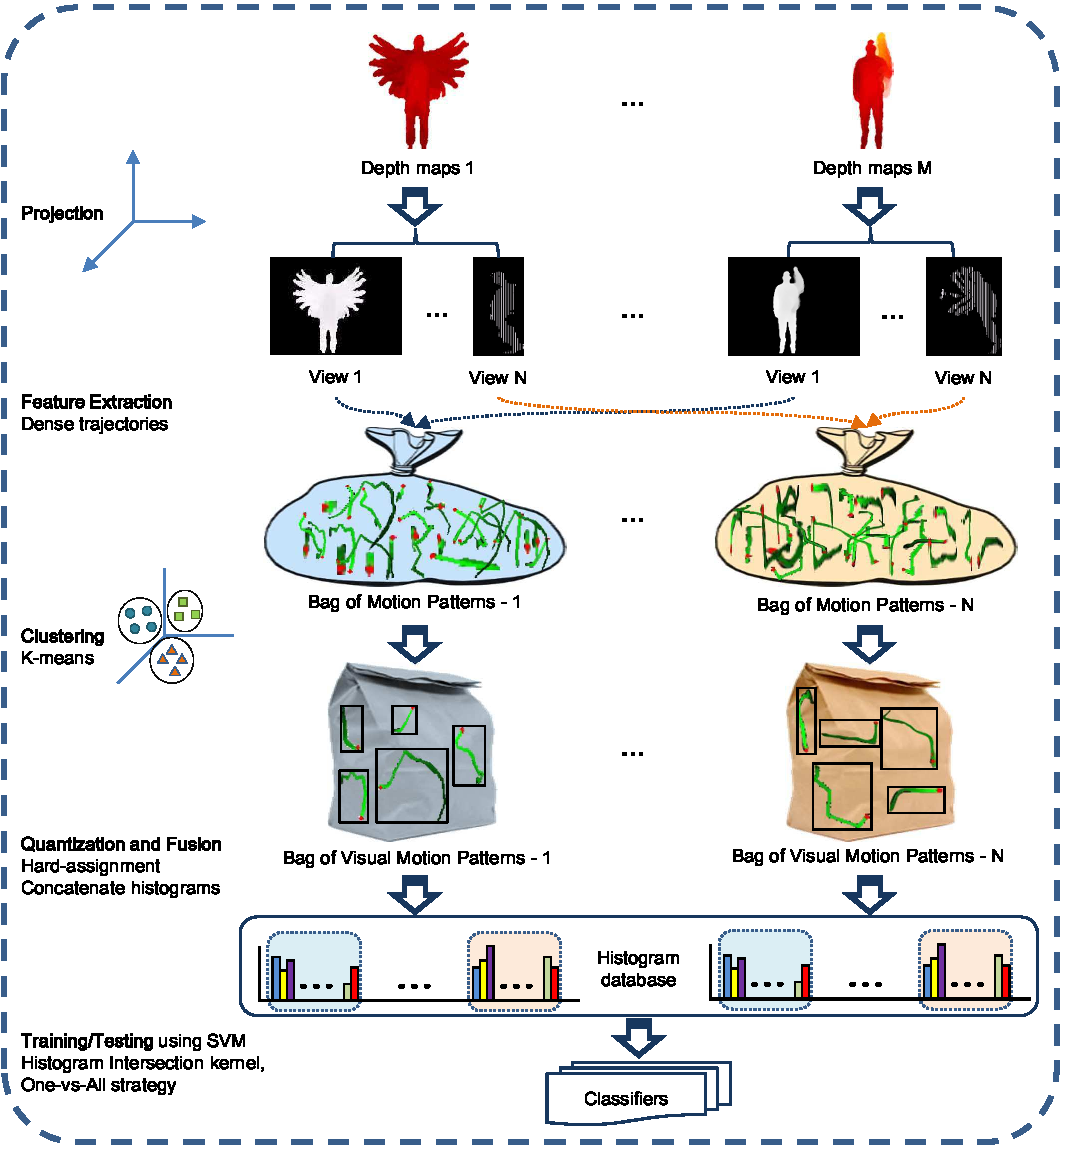
\includegraphics[width=0.75\textwidth]{Figures/Framework3D.pdf} %
	\caption{Our Framework Overview}
	\label{Figure_FrameworkOverview}
\end{figure*}

\section{Action Recognition Framework}
\label{Section_Framework}
In this section, we present a unified action recognition framework on depth data.
We extract discriminative motion patterns based on observation views, and then apply a bag-of-words model to compute feature vectors for the feature fusion scheme.
The motivation for using a bag-of-words model to action recognition is to handle the variable number of motion patterns produced by arbitrary movements from various subjects.
The fused feature vectors computed from a bag-of-words model are inputs of classifiers in training and testing phases.
Following subsections provide concise descriptions about processes in our framework.

\paragraph{\textbf{Projection}}
A key problem is the appropriate action representation to capture discriminative motion patterns effectively.
Currently, capturing the motion patterns has not been achieved specific successes on 3D data in comparison with 2D data.
Therefore, at this step, we try to present each 3D action by a set of 2D actions.
To do that, \textit{M} depth maps are projected onto \textit{N} view planes to obtain corresponding 2D motion representations.
After the projection, each 2D motion representation is abstracted by several local motion patterns.

\paragraph{\textbf{Feature Extraction}}
In order to capture discriminative motion patterns on the 2D motion representations, we adopt the trajectory-based approach.
With this approach, we can handle the challenges from human body segmentation as well as skeleton extraction.
Trajectory-aligned descriptors are then calculated on the extracted trajectories to build \textit{N} ``bags of motion patterns'' corresponding to \textit{N} views.

\paragraph{\textbf{Clustering}}
The clustering step is to convert a ``bag of motion patterns'' from training dataset to a ``bag of visual motion patterns''.
A visual motion pattern can be considered as a representative of several similar motion patterns.
One clustering method (e.g. k-means) can be applied over all the motion patterns.
Visual motion patterns are then defined as the centers of the learned clusters.
The number of the clusters is the size of ``bag of visual motion patterns''.

\paragraph{\textbf{Quantization and Fusion}}
To represent an action with captured motion patterns, we map each ``motion pattern'' to a certain ``visual motion pattern'' through the matching process.
Afterwards, the histogram of the visual motion patterns is generated to represent action on a corresponding view.
After that, the histograms generated from all views are concatenated to form a larger feature vector as input to a classifier.
Since each individual feature vector has the same meaning, the feature fusion can guarantee the effectiveness to represent action.

\paragraph{\textbf{Training and testing}}
After the final feature representations are generated, we separate them into two histogram databases for training and testing phases.
We use a machine learning method such as Support Vector Machine (SVM) for classification.
In practice, we use the precomputed-kernel technique with the histogram intersection kernel for this process.
Besides, we perform the one-vs-all strategy for multi-class classification.

Our proposed trajectory-based approach is compared with the state-of-the-art methods for human action recognition on depth data.
Actually, our approach does not count skeleton extraction, which is used as an important factor in some works, such as \cite{wang2012mining, yang2012eigenjoints, luo2013group}.
In fact, extracting skeleton exactly is still an completely unsolved problem, due to the challenges, such as cluttered background, hardware quality, camera motion, so on.

\section{Proposed Method}
\label{Section_ProposedMethod}

This paper presents an effective method for action recognition on depth video by exploiting the discriminative motion patterns.
As mentioned in section \ref{Section_Framework}, to support the aim, we analyze each 3D action to a set of 2D actions and leverage the trajectory-based approach to capture effectively the discriminative motion patterns.
In this section, we provide a description of our proposed method to obtain 2D motion representations from various views.
In addition, we present briefly the dense trajectory-based feature proposed by Wang.H et al. \cite{wang2011densetraj}, which has been demonstrated state-of-the-art at action recognition.
Related parts, such as: dense sampling, tracking and feature descriptors are also referred to.

\begin{figure}[h]
	\centering
	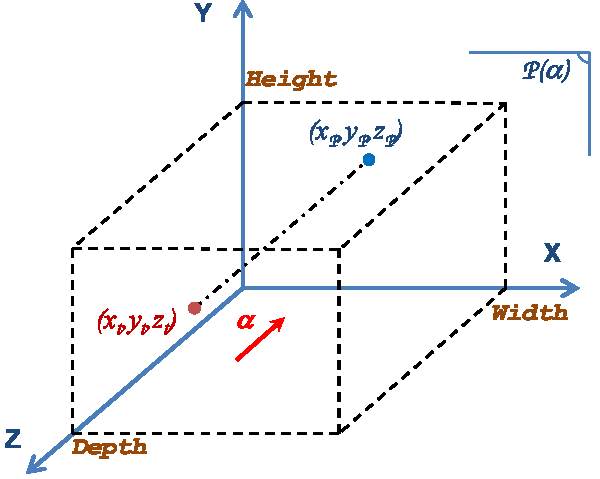
\includegraphics[width=0.47\textwidth]{Figures/Figure_PointProjection.pdf} %
	\caption{\label{lbl:Figure_PointProjection}An illustration of the projection. Point $P_\mathcal{P} = (x_\mathcal{P},y_\mathcal{P},z_\mathcal{P})$ is the projection of point $P_t  = (x_t,y_t,z_t)$ along a view direction $\alpha$ onto a view plane $\mathcal{P}(\alpha)$.}
\end{figure}

\subsection{2D Motion Representations}

Our proposed method to exploit discriminative motion patterns for human action recognition on depth video is as follow.
At first, 2D motion representations are formed from the sequence of depth maps, as illustrated in figure \ref{Figure_ProposedMethod}.
At this step, to obtain an intensity video from a view direction $\alpha$, corresponding to a view plane $\mathcal{P}(\alpha): ax + by + cx + d = 0$, in each depth map $t$, each point $P_t = (x_t,y_t,z_t)$ is projected to $P_\mathcal{P} = (x_\mathcal{P},y_\mathcal{P},z_\mathcal{P})$ on the view plane $\mathcal{P}(\alpha)$, see in figure \ref{lbl:Figure_PointProjection}, by:

\begin{equation}
	P_t = (x_t,y_t,z_t)\xrightarrow{\mathcal{P}(\alpha)}P_\mathcal{P} = (x_\mathcal{P},y_\mathcal{P},z_\mathcal{P})
\end{equation}

where,
\begin{equation}
	x_\mathcal{P} = x_t - \frac{ax_t + by_t + cz_t + d}{a^2 + b^2 + c^2}a
\end{equation}
\begin{equation}
	y_\mathcal{P} = y_t - \frac{ax_t + by_t + cz_t + d}{a^2 + b^2 + c^2}b
\end{equation}
\begin{equation}
	z_\mathcal{P} = z_t - \frac{ax_t + by_t + cz_t + d}{a^2 + b^2 + c^2}c
\end{equation}
And the intensity value $v$ at the projected point $P_\mathcal{P}$ is computed by:
\begin{equation}
	v(P_\mathcal{P}) = \frac{ax_t + by_t + cz_t + d}{\sqrt{a^2 + b^2 + c^2}}
\end{equation}
So, given a set of 3D points $\mathcal{S}(t) = \{(x_t,y_t,z_t)\vert(x_t,y_t,z_t) \in t\}$, we have a projection $\mathcal{S}_\alpha(t) = \{(x_\mathcal{P},y_\mathcal{P},z_\mathcal{P})\vert(x_\mathcal{P},y_\mathcal{P},z_\mathcal{P}) \in \mathcal{P}(\alpha)\}$. Therefore, a set of the projections obtained from a given sequence of M depth maps under a view direction $\alpha$ is an expected intensity video $\mathcal{R}(\alpha) = \{\mathcal{S}_\alpha(t) \vert t=\overline{1..M}\}$. Each intensity video obtained from the corresponding projection onto the sequence of depth maps can be regarded as a 2D transformed video of action in depth video.

In particular, we choose three representations to represents for three view directions: front, side, and top in 3D space, corresponding to three view planes, respectively: $Oxy$, $Oyz$ and $Ozx$. With these view directions, the corresponding projections are respectively:
\begin{equation}
	\mathcal{S}_\text{front}(t) = \{(x_t,y_t,0)\vert(x_t,y_t,0) \in \mathcal{P}:z=0\}
\end{equation}
\begin{equation}
	\mathcal{S}_\text{side}(t) = \{(0,y_t,z_t)\vert(0,y_t,z_t) \in \mathcal{P}:x=0\}
\end{equation}
\begin{equation}
	\mathcal{S}_\text{top}(t) = \{(x_t,0,z_t)\vert(x_t,0,z_t) \in \mathcal{P}:y=0\}
\end{equation}
And the corresponding intensity values in the three projections are, respectively:
\begin{equation}
	v(P_\text{front}) = z_t
\end{equation}
\begin{equation}
	v(P_\text{side}) = x_t
\end{equation}
\begin{equation}
	v(P_\text{top}) = y_t
\end{equation}

\subsection{Dense trajectories}
% - Giới thiệu khái quát về dense trajectories
Trajectories provide a compact representation of motion information in video.
Trajectories from intensity videos can be used for multimedia event detection (MED), video mining, action classification and so on.
Trajectory extraction much depends on both processes: sampling and tracking.
Some concerned methods, such as \cite{matikainen2009trajectons, messing2009activity} used KLT tracker \cite{lucas1981iterative}, or \cite{sun2009hierarchical} matched SIFT descriptors between consecutive frames to obtain feature trajectories.
Recently, the dense trajectory-based motion feature proposed by \cite{wang2011densetraj} has achieved the state-of-the-art performances on MED systems, such as, segment-based system \cite{phan2014multimedia} on TRECVID MED 2010, 2011, or AXES \cite{oneata2012axes}, and BBNVISER \cite{natarajan2012bbn} on TRECVID MED 2012.

In order to obtain trajectories, there are two important steps: sampling and tracking. \cite{wang2011densetraj} propose sampling on a dense grid with a step size of 5 pixels. The sampling is performed at multiple scales with a factor of $1/\sqrt{2}$. Then, tracking is the next step to form trajectories. At each scale, in frame \textit{t}, each point \textit{$P_t = (x_t, y_t)$} is tracked to point \textit{$P_{t+1} = (x_{t+1}, y_{t+1})$} in next frame \textit{t+1} by:
\begin{equation}
	\textit{$P_{t+1} = (x_{t+1}, y_{t+1}) = (x_t, y_t) + (M*\omega)|_{(\bar{x}_t,\bar{y}_t)} $},
\end{equation}
where \textit{$\omega = (u_t, v_t)$} denotes the dense optical flow field, \textit{M} is the kernel of median filtering, and \textit{$(\bar{x}_t,\bar{y}_t)$} is the rounded position of \textit{$P_t$}. The algorithm of \cite{farneback2003two} is adopted to compute the dense optical flow. And to avoid a drifting problem, a suitable value of trajectory length is set to 15 frames. Besides, trajectories with sudden changes are removed.

After extracting trajectories, two kinds of descriptors: a trajectory shape descriptor and a trajectory-aligned descriptor can be adopted. In our experiments, we only use trajectory-aligned descriptors including the HOG \cite{dalal2005histograms}, the Histogram of Optical Flow (HOF) \cite{laptev2008learning}, and the Motion Boundary Histogram (MBH) \cite{dalal2006human}. HOG captures local appearance information, while HOF and MBH encode local motion pattern. The descriptors are computed within a space-time volume ($N \times N$ spatial pixels and $L$ temporal frames) around the trajectory. This volume is divided into a 3D grid (spatially $n_\sigma \times n_\sigma$ grid and temporally $n_\tau$ segments). The default settings of these parameters are $N$ = 32 pixels, $L$ = 15 frames, $n_\sigma$ = 2, and $n_\tau$ = 3.

\iffalse
\paragraph{Trajectory Shape Descriptor}This descriptor describes the shape of a trajectory in the simplest way. Given a trajectory of length L, its shape is concatenated by a sequence of displacement vectors \textit{$S = (\Delta P_t, ..., \Delta P_{t+L-1})$}, where \textit{$\Delta P_t = P_{t+1} - P_t = (x_{t+1} - x_t, y_{t+1} - y_t)$}. In order to make the descriptor invariant to scale changes, the final result is then achieved by normalizing the shape vector by the overall magnitude of the displacement vectors:

\begin{equation}
	\textit{$\bar{S} = \frac{(\Delta P_t, ..., \Delta P_{t+L-1})}{\sum_{k=t}^{t+L-1}\|\Delta P_k\|}$},
\end{equation}
\fi
%\paragraph{Trajectory-aligned Descriptor}
%In order to capture the local motion and appearance around a trajectory, three kinds of descriptors have been employed: the HOG \cite{dalal2005histograms}, the Histogram of Optical Flow (HOF) \cite{laptev2008learning}, and the Motion Boundary Histogram (MBH) \cite{dalal2006human}. For HOG, orientation information is quantized into 8-bin histogram. HOF is 9-bin histogram. Since the feature of a trajectory is calculated and concatenated from sub-volumes of a 3D volume, the final representation has 96 dimensions for HOG and 108 dimensions for HOF. MBH descriptor computes derivatives on both horizontal and vertical components of optical flow $I_\omega = (I_x. I_y)$. Similar to HOG descriptor, the orientation information is quantized into 8-bin histogram. Since the motion information is combined along two directions, the final representation is $96 \times 2 = 192$-bin histogram. By presenting gradient of optical flow, MBH descriptor is able to suppress global motion information and only keep local relative changes in pixels.

According to the authors \cite{laptev2008learning, wang2011densetraj, wang2009evaluation, liu2009recognizing}, all the three descriptors have shown the effectiveness for action recognition. The experimental settings for these descriptors are based on an empirical study showed in \cite{wang2011densetraj}. We also conduct our experiment on all the three descriptors when compared to the depth-based state-of-the-art methods.

\begin{figure*}[ht]
	\centering
	\resizebox{\textwidth}{!}{
		% Table generated by Excel2LaTeX from sheet 'Sheet3'
		\begin{tabular}{ccccc}
			
			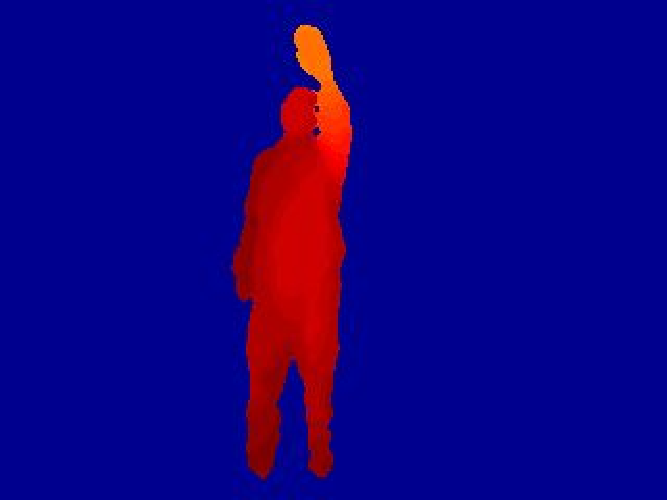
\includegraphics[width=0.4\columnwidth]{Figures/MSRAction3D_higharmwave.pdf} &          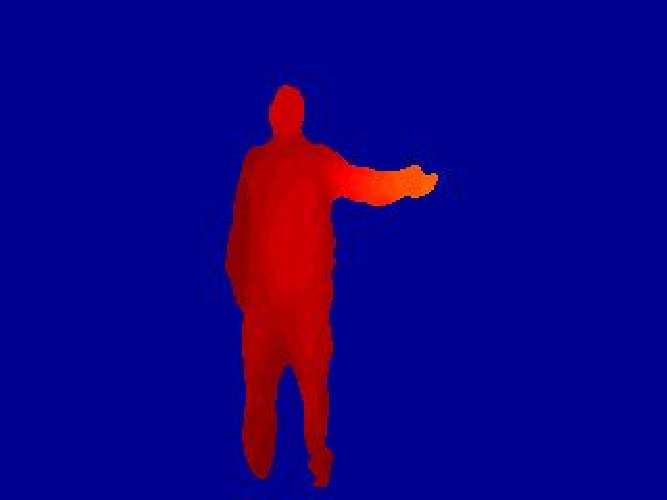
\includegraphics[width=0.4\columnwidth]{Figures/MSRAction3D_horizontalarmwave.pdf} &          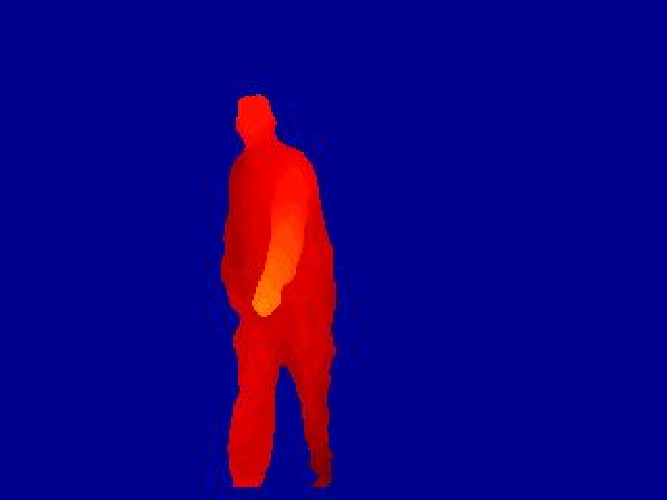
\includegraphics[width=0.4\columnwidth]{Figures/MSRAction3D_hammer.pdf} &          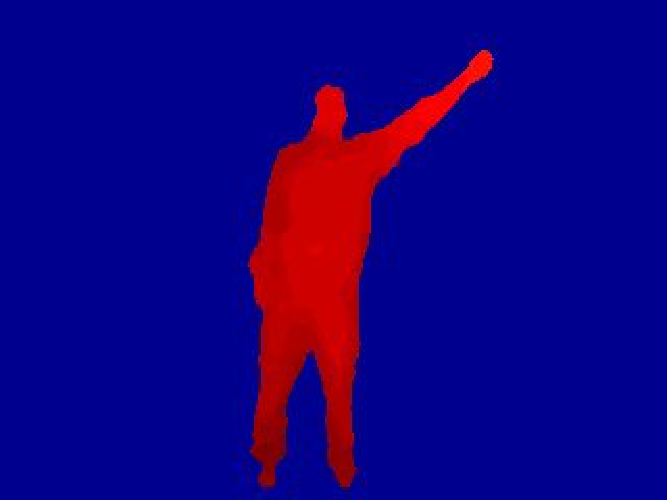
\includegraphics[width=0.4\columnwidth]{Figures/MSRAction3D_handcatch.pdf} &          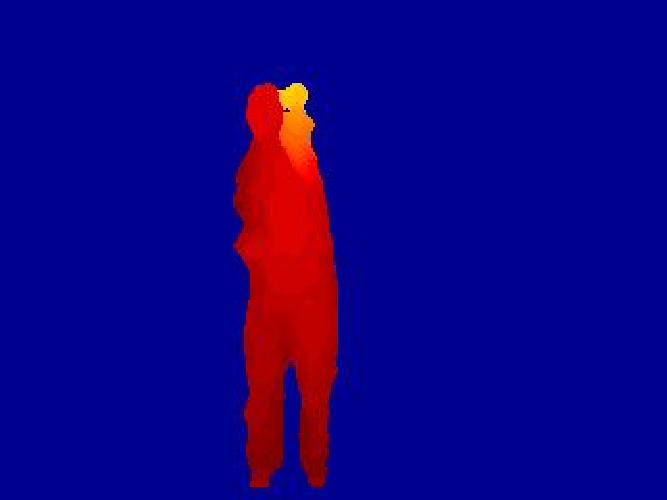
\includegraphics[width=0.4\columnwidth]{Figures/MSRAction3D_forwardpunch.pdf}\\
			
			1. High arm wave &          2. Horizontal arm wave &          3. Hammer &          4. Hand catch &          5. Forward punch\\
			
			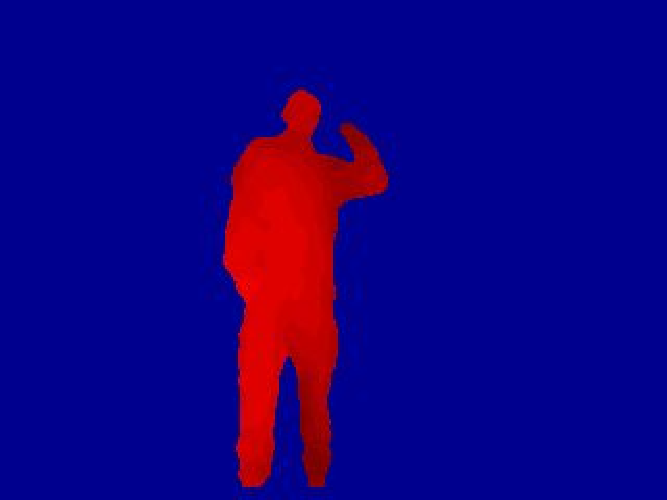
\includegraphics[width=0.4\columnwidth]{Figures/MSRAction3D_highthrow.pdf} &          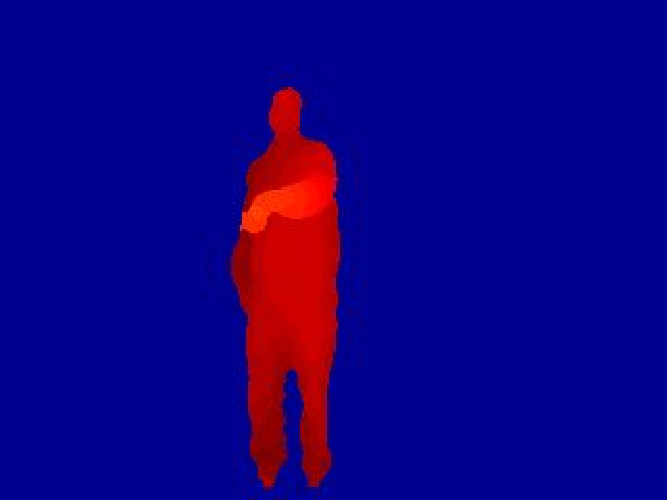
\includegraphics[width=0.4\columnwidth]{Figures/MSRAction3D_drawx.pdf} &          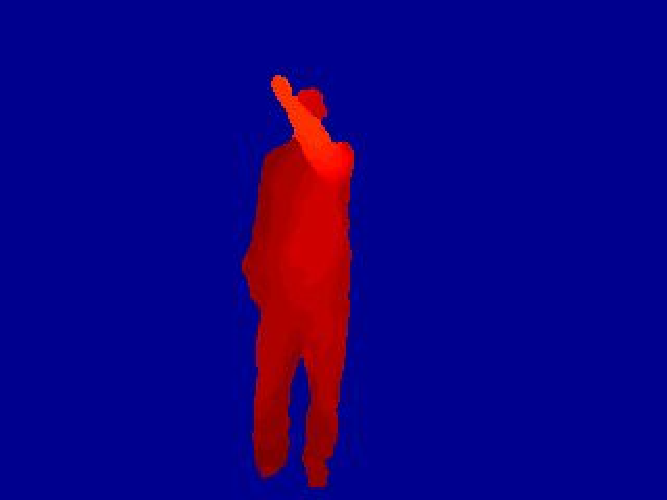
\includegraphics[width=0.4\columnwidth]{Figures/MSRAction3D_drawtick.pdf} &          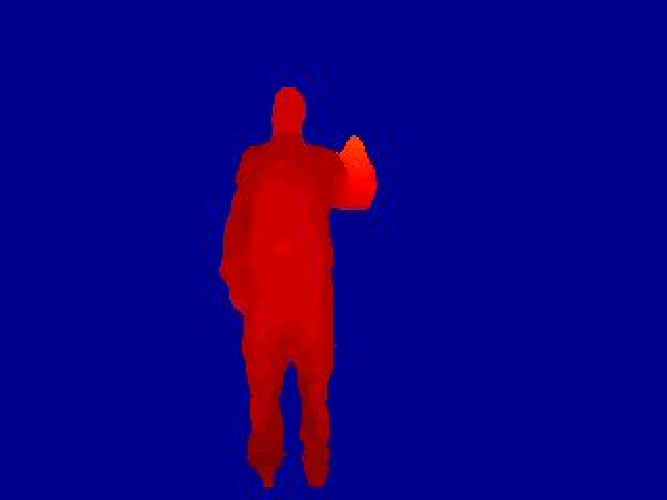
\includegraphics[width=0.4\columnwidth]{Figures/MSRAction3D_drawcircle.pdf} &          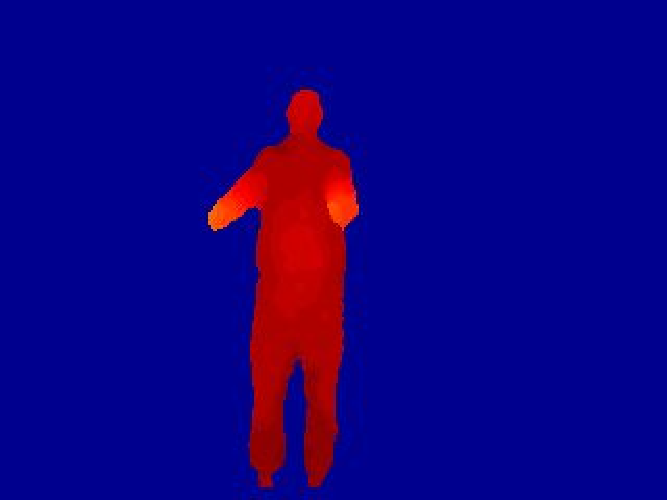
\includegraphics[width=0.4\columnwidth]{Figures/MSRAction3D_handclap.pdf} \\
			
			6. High throw &          7. Draw X &          8. Draw tick &           9. Draw circle &          10. Hand clap\\
			
			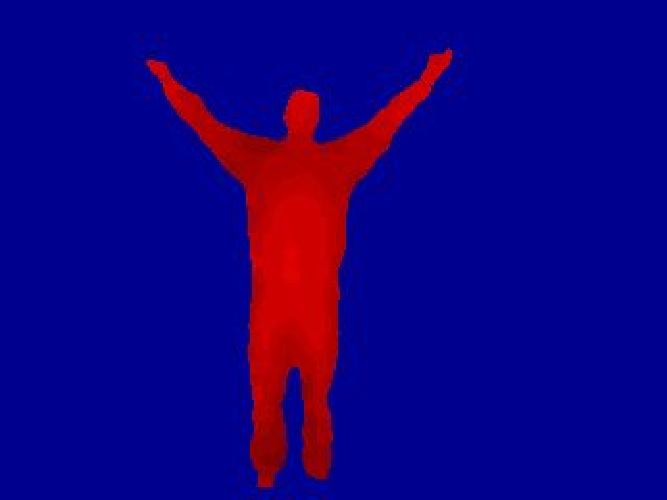
\includegraphics[width=0.4\columnwidth]{Figures/MSRAction3D_twohandwave.pdf} &          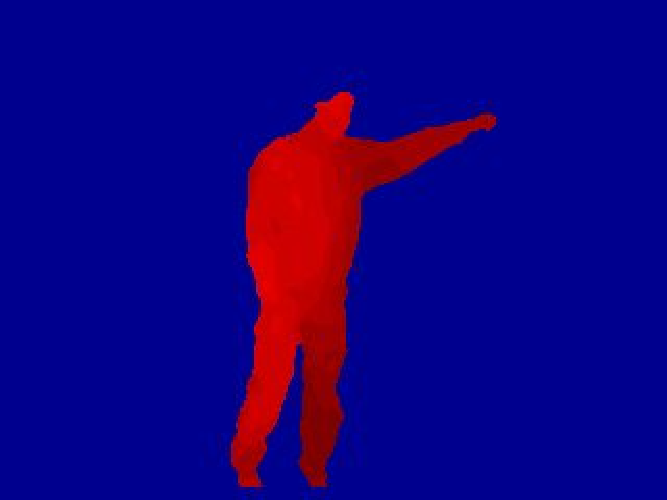
\includegraphics[width=0.4\columnwidth]{Figures/MSRAction3D_sideboxing.pdf} &          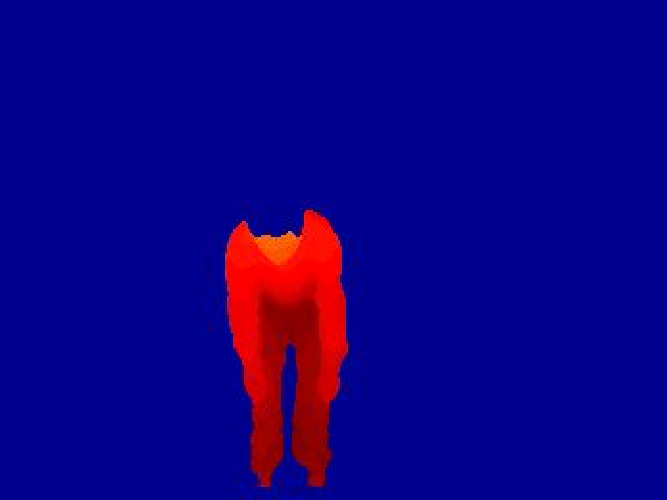
\includegraphics[width=0.4\columnwidth]{Figures/MSRAction3D_bend.pdf} &          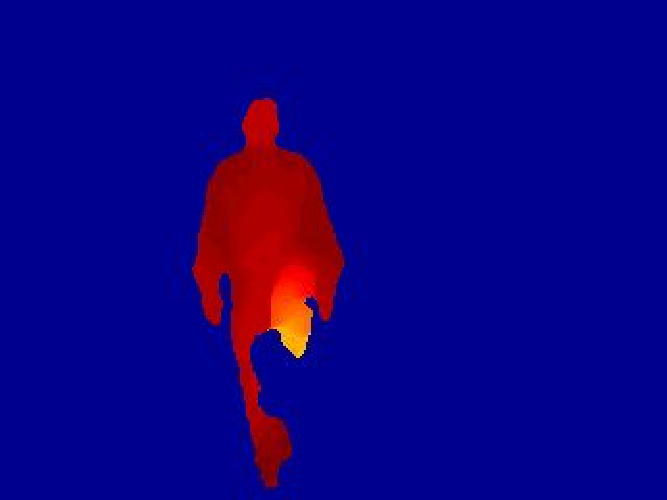
\includegraphics[width=0.4\columnwidth]{Figures/MSRAction3D_forwardkick.pdf} &          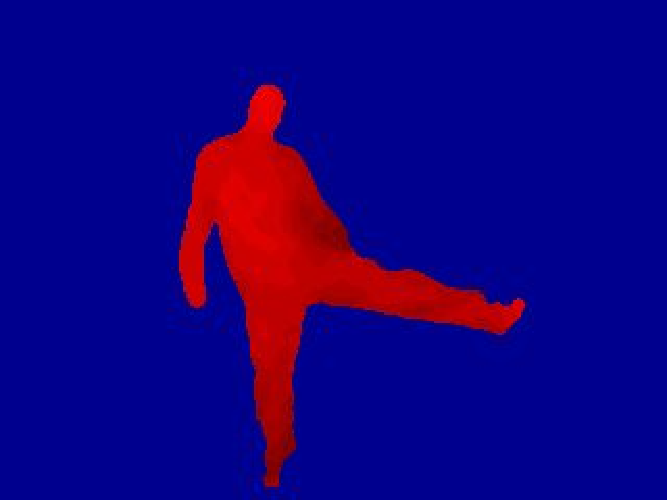
\includegraphics[width=0.4\columnwidth]{Figures/MSRAction3D_sidekick.pdf} \\
			
			11. Two hand wave &          12. Side-boxing &         13. Bend &          14. Forward kick &          15. Side kick\\
			
			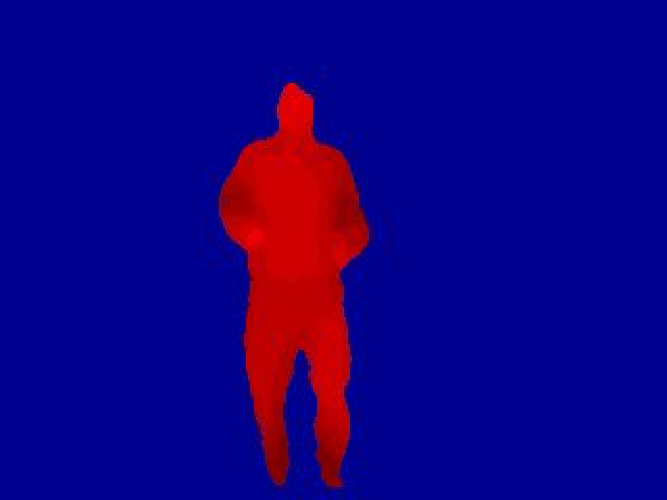
\includegraphics[width=0.4\columnwidth]{Figures/MSRAction3D_jogging.pdf} &		
			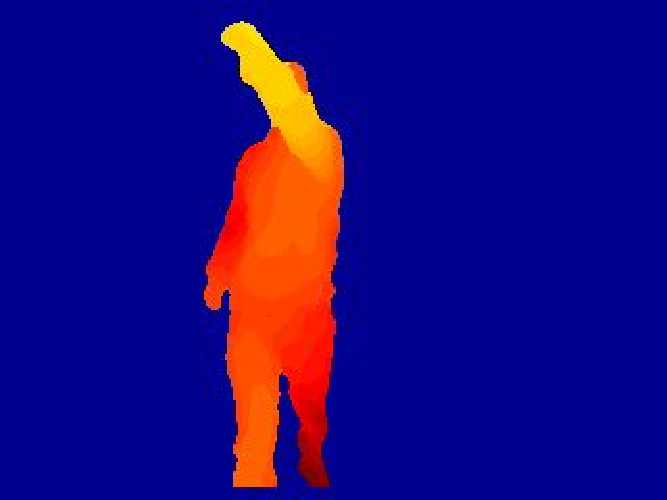
\includegraphics[width=0.4\columnwidth]{Figures/MSRAction3D_tennisswing.pdf} &          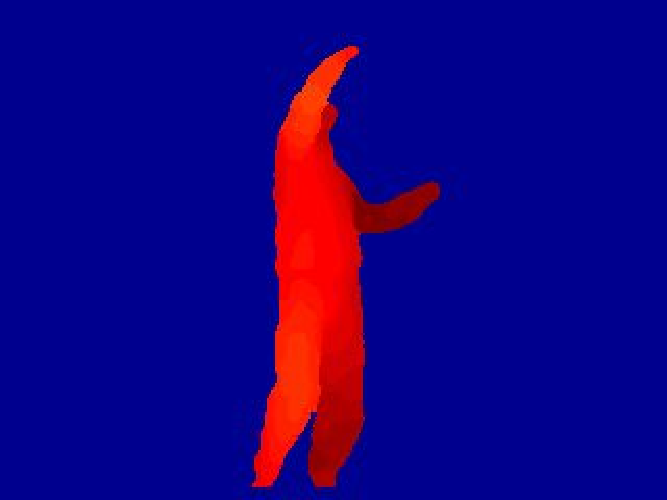
\includegraphics[width=0.4\columnwidth]{Figures/MSRAction3D_tennisserve.pdf} &          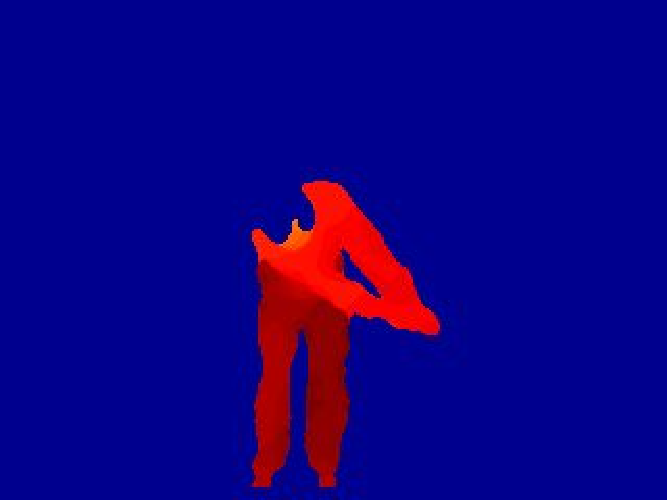
\includegraphics[width=0.4\columnwidth]{Figures/MSRAction3D_golfswing.pdf} &          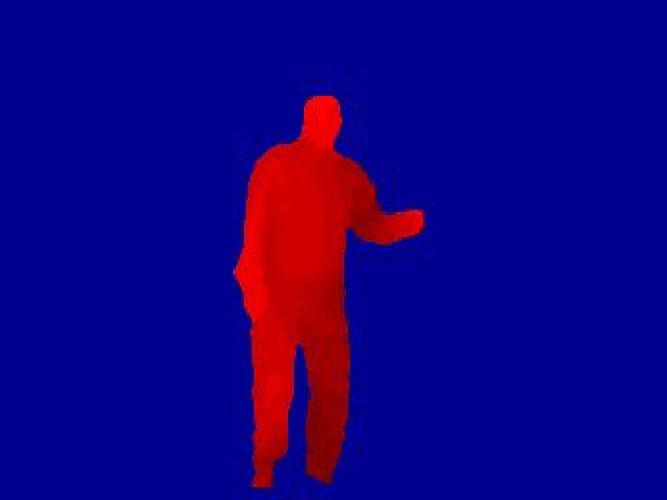
\includegraphics[width=0.4\columnwidth]{Figures/MSRAction3D_pickupandthrow.pdf} \\
			
			16. Jogging &         17. Tennis swing &          18. Tennis serve &          19. Golf swing &          20. Pick up \& Throw \\
			
		\end{tabular}  
		
	}
	\caption{Example frames for twenty actions from MSR Action 3D dataset \cite{li2010action}.}
	\label{Figure_ExampleFrames_MSRAction3D}
\end{figure*}

\section{Experiments}
\label{Section_Experiments}
This section presents the experimental results for applying our proposed approach on MSR Action 3D dataset, MSR Gesture 3D dataset, and 3D Action Pairs dataset.
For analysis, we concentrate on MSR Action 3D dataset to explain experimental results.
For MSR Gesture 3D dataset and 3D Action Pairs dataset, we only show the final results.
All experimental results are reported under the settings mentioned in section \ref{Subsection_ExperimentalSettings}.
In comparison with the state-of-the-art methods, our reported result is calculated on concatenating feature representations from the combinations of three views: front, side and top.
%In addition, an evaluation related to selecting compensation information from the three views will be also mentioned.
All the results are compared in terms of recognition accuracy.
The best performance is highlighted in bold.

\subsection{Framework Settings}
\label{Subsection_ExperimentalSettings}

In this section, we provide a experimental settings used in our framework, as described in section \ref{Section_Framework}.

\paragraph{\bf \textit{Projection}}
Based on works \cite{li2010action, yang2012recognizing}, we select three views: front, side and top to project sequence of depth maps onto.
Results obtained from the projections are three 2D motion representations.

\paragraph{\bf \textit{Feature Extraction}}
We use the application available online\footnote{http://lear.inrialpes.fr/$\sim$wang/dense\_trajectories} to extract dense trajectories and calculate aligned-descriptors (i.e. MBH, HOG and HOF) for each 2D motion representation.
Experimental results reported in section \ref{Section_Experiments} attach to the MBH descriptor.
The HOG, HOF descriptors will be mentioned in the section \ref{Section_Discussion}.

\paragraph{\bf \textit{Clustering}}
%To represent 2D transformed videos, the BoW model is applied.
At this step, we create three codebooks (i.e. three bags of visual motion patterns), corresponding to three views: front, side and top.
Each codebook contains 2000 visual codewords which are built by using K-means algorithm with Euclidean distance to cluster dense trajectory motion features.
The number of visual codewords is selected due to the purpose of the stable and unified framework on all benchmark datasets.

\paragraph{\bf \textit{Quantization and Fusion}}
In order to quantize a large number of dense trajectory motion features extracted at step {\it Feature Extraction}, we apply the hard-assignment strategy.
With this strategy, each feature vector can be assigned to a codeword using Euclidean distance or rejected as an outlier.
After BoW features are quantized for 2D motion representations, they are concatenated to form feature representations for corresponding actions.
%Based on our previous experiments, we have chosen early fusion as a major fusion scheme.
The feature representations concatenated from the BoW features, then, are separated into two histogram databases for training and testing phases.

\paragraph{\bf \textit{Training and Testing}}
In order to classify actions, in our implementation, we use the libSVM library \cite{chang2011libsvm} published online by author\footnote{http://www.csie.ntu.edu.tw/$\sim$cjlin/libsvm/}.
We adopt the format requirements of the library to synchronize the annotation and the data.
We apply histogram intersection kernel:
\begin{equation}
K(a,b) = \sum_{i=1}^{n}\min(a_i,b_i), a_i \geq 0, b_i \geq 0
\end{equation}
to compute matching matrices before we do training and testing with SVM.
For testing, the one-vs-all strategy is used.
Predicted value of each action is defined as the maximum score obtained from all the classifiers.
This score shows that a human action is confused with another or not.



\subsection{MSR Action 3D Dataset}

\subsubsection{A Brief Introduction}
This dataset \cite{li2010action} contains 20 actions, as showed in figure \ref{Figure_ExampleFrames_MSRAction3D}. Actions are performed by ten subjects for two or three times in the context of game console interaction. In total, there are 567 sequences of depth maps. The depth maps are shot at frame rate of 15 fps. The size of the depth map is $320 \times 240$ to ensure processing efficiency.

\begin{table}[h]
	\begin{center}
		\resizebox{0.47\textwidth}{!}{%
			% Table generated by Excel2LaTeX from sheet 'Sheet3'
			\begin{tabular}{c|c|c}
				
				{\bf Action Subset 1} & {\bf Action Subset 2} & {\bf Action Subset 3} \\
				{\bf(AS1)} & {\bf(AS2)} & {\bf(AS3)} \\
				\hline
				horizontal arm wave &  high arm wave &     high throw \\
				
				hammer &     hand catch &   forward kick \\
				
				forward punch &         draw x &      side kick \\
				
				high throw &      draw tick &        jogging \\
				
				hand clap &    draw circle &   tennis swing \\
				
				bend &  two hand wave &   tennis serve \\
				
				tennis serve &    side-boxing &     golf swing \\
				
				pick up \& throw &   forward kick & pick up \& throw \\
				
			\end{tabular} %
		}
	\end{center}
	\caption{\label{lbl:3ActionSubsets}The three action subsets used in the experiments}
\end{table}

In order to conduct a fair comparison, we use the same experimental settings as \cite{li2010action, yang2012eigenjoints, vieira2012stop, wang2012mining, wang2012robust, yang2012recognizing, xia2013spatio, oreifej2013hon4d, luo2013group}.
In the settings, the dataset is divided into three action subsets. Each subset has 8 actions (Table \ref{lbl:3ActionSubsets}).
The two subsets AS1 and AS2 present that grouped actions have similar movements.
The subset AS3 groups complex actions together.
For instance, action \textit{hammer} seems to be confused with action \textit{forward punch} in AS1 or similar movements between action \textit{hand catch} and action \textit{side boxing} in AS2.
As for each subset, we select half of the subjects as training and the rest as testing (i.e. cross subject test).

\begin{figure}[h]
	\centering
	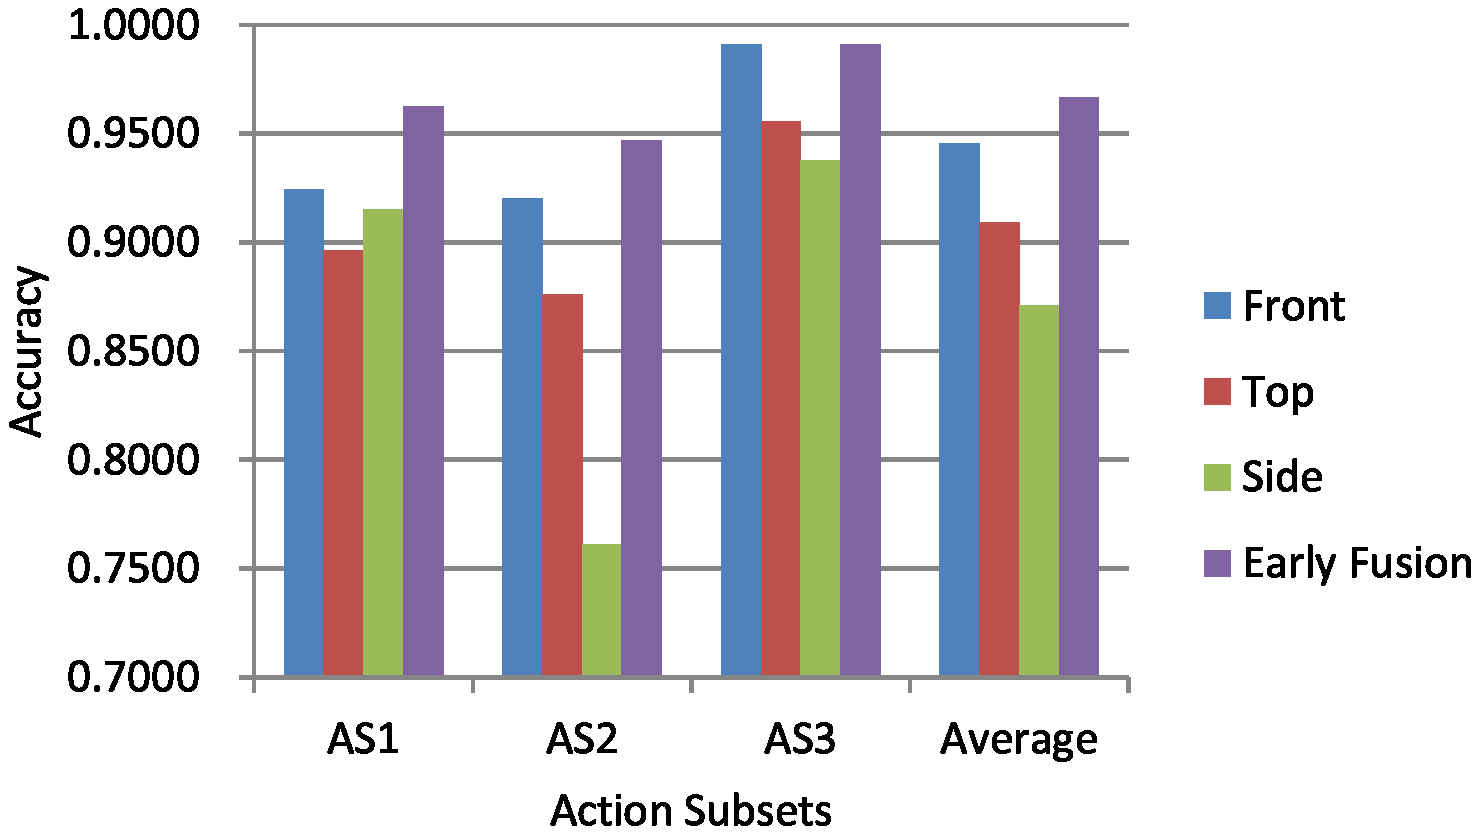
\includegraphics[width=\columnwidth]{Figures/Chart_EarlyFusion_AS123_MBH.pdf}
	\caption{A comparison of recognition accuracy between the separated views and the all view-based combination.}
	\label{lbl:Figure_EarlyFusion_AS123_MBH}
\end{figure}

\subsubsection{Recognize Actions from Single-View}

In this part, we evaluate the dense trajectory-based approach for action recognition under observing actions from single-view.
A straightforward view is front view.
In order to obtain action presentation on front view from depth video, a simple way is to consider depth value as intensity value.
Table \ref{lbl:AS123ConfusionMatrix} shows three confusion matrices corresponding to evaluations on three action subsets from MSR Action 3D dataset.
Consider results reported in table \ref{lbl:AS123ConfusionMatrix}, we found that two subsets AS1, AS2 contain many confused actions. For example, \textit{hammer} (a03) and \textit{forward punch} (a05) in AS1, or \textit{side-boxing} (a12) and \textit{hand catch} (a04) in AS2.
When analyzing such actions, we found that the main cause is due to similar movements of actions in the same view direction.
That is reason why we need compensate motion information from other views (e.g. side view and top view).

\begin{figure}[h]
	\centering
	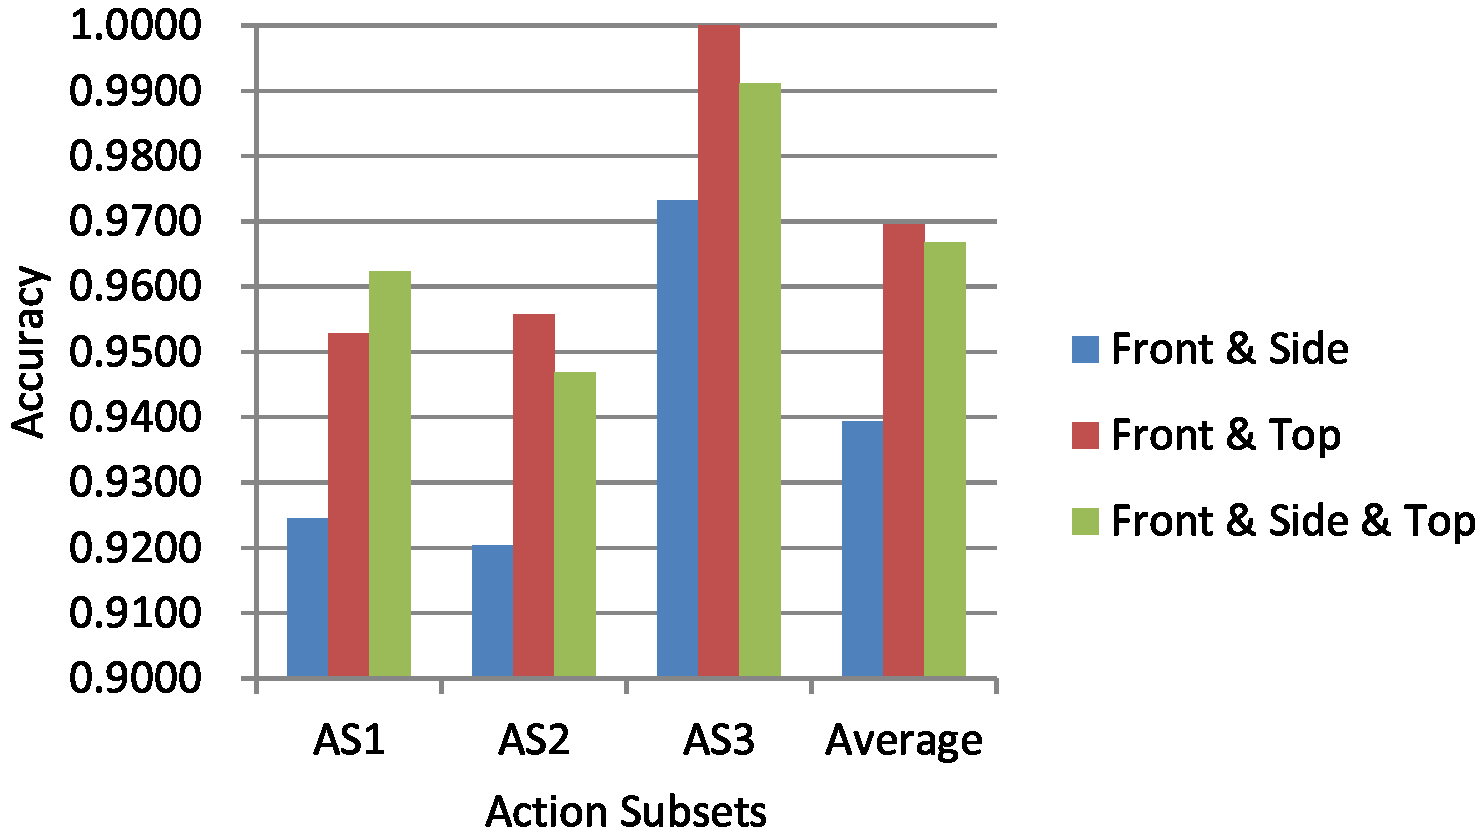
\includegraphics[width=\columnwidth]{Figures/Chart_RoleOfRepresentations.pdf}
	\caption{Comparison of recognition accuracy on combinations of intensity representations on MSR Action 3D dataset.}
	\label{Figure_CombinationsFRONTSIDETOP}
\end{figure}

\begin{table}[h]
	%	\resizebox{\textwidth}{!}{
	\begin{center}
		\subfloat[Action Subset 1 \label{lbl:ConfMatAS1}]{ %
			% Table generated by Excel2LaTeX from sheet 'Experiment-MSRDaily3D'
			\resizebox{\columnwidth}{!}{
				\begin{tabular}{c|c|c|c|c|c|c|c|c|}
					\multicolumn{1}{c}{~}& \multicolumn{1}{c}{\bf a02} & \multicolumn{1}{c}{\bf a03} & \multicolumn{1}{c}{\bf a05} & \multicolumn{1}{c}{\bf a06} & \multicolumn{1}{c}{\bf a10} & \multicolumn{1}{c}{\bf a13} & \multicolumn{1}{c}{\bf a18} & \multicolumn{1}{c}{\bf a20} \\
					\hhline{~--------}
					{\bf a02} & \color{white}{\bf 0.83}\cellcolor[gray]{.2} & 0 & {\bf 0.17}\cellcolor[gray]{.8} & 0 & 0 & 0 & 0 & 0 \\
					\hhline{~--------}
					{\bf a03} & 0 & \color{white}{\bf 0.92}\cellcolor[gray]{.1} & {\bf 0.08}\cellcolor[gray]{.9} & 0 & 0 & 0 & 0 & 0 \\
					\hhline{~--------}
					{\bf a05} & 0 & {\bf 0.36}\cellcolor[gray]{.6} & \color{white}{\bf 0.64}\cellcolor[gray]{.4} & 0 & 0 & 0 & 0 & 0 \\
					\hhline{~--------}
					{\bf a06} & 0 & 0 & 0 & \color{white}{\bf 1.0}\cellcolor[gray]{.0} & 0 & 0 & 0 & 0 \\
					\hhline{~--------}
					{\bf a10} & 0 & 0 & 0 & 0 & \color{white}{\bf 1.0}\cellcolor[gray]{.0} & 0 & 0 & 0 \\
					\hhline{~--------}
					{\bf a13} & 0 & 0 & 0 & 0 & 0 & \color{white}{\bf 1.0}\cellcolor[gray]{.0} & 0 & 0 \\
					\hhline{~--------}
					{\bf a18} & 0 & 0 & 0 & 0 & 0 & 0 & \color{white}{\bf 1.0}\cellcolor[gray]{.0} & 0 \\
					\hhline{~--------}
					{\bf a20} & 0 & 0 & 0 & 0 & 0 & {\bf 0.07}\cellcolor[gray]{.9} & 0 & \color{white}{\bf 0.93}\cellcolor[gray]{.1} \\
					\hhline{~--------}
				\end{tabular} %
			} %
		}
		
		\subfloat[Action Subset 2 \label{lbl:ConfMatAS2}]{
			% Table generated by Excel2LaTeX from sheet 'Experiment-MSRDaily3D'
			\resizebox{\columnwidth}{!}{
				\begin{tabular}{c|c|c|c|c|c|c|c|c|}
					\multicolumn{1}{c}{~}& \multicolumn{1}{c}{\bf a01} & \multicolumn{1}{c}{\bf a04} & \multicolumn{1}{c}{\bf a07} & \multicolumn{1}{c}{\bf a08} & \multicolumn{1}{c}{\bf a09} & \multicolumn{1}{c}{\bf a11} & \multicolumn{1}{c}{\bf a12} & \multicolumn{1}{c}{\bf a14} \\
					\hhline{~--------}
					{\bf a01} & \color{white}{\bf 1.0}\cellcolor[gray]{.2} & 0 & 0 & 0 & 0 & 0 & 0 & 0 \\
					\hhline{~--------}
					{\bf a04} & {\bf 0.08}\cellcolor[gray]{.9} & \color{white}{\bf 0.84}\cellcolor[gray]{.2} & {\bf 0.08}\cellcolor[gray]{.9} & 0 & 0 & 0 & 0 & 0 \\
					\hhline{~--------}
					{\bf a07} & 0 & 0 & \color{white}{\bf 0.79}\cellcolor[gray]{.2} & {\bf 0.07}\cellcolor[gray]{.9} & {\bf 0.07}\cellcolor[gray]{.9} & 0 & {\bf 0.07}\cellcolor[gray]{.9} & 0 \\
					\hhline{~--------}
					{\bf a08} & 0 & 0 & 0 & \color{white}{\bf 1.0}\cellcolor[gray]{.0} & 0 & 0 & 0 & 0 \\
					\hhline{~--------}
					{\bf a09} & 0 & 0 & 0 & {\bf 0.13}\cellcolor[gray]{.9} & \color{white}{\bf 0.87}\cellcolor[gray]{.1} & 0 & 0 & 0 \\
					\hhline{~--------}
					{\bf a11} & 0 & 0 & 0 & 0 & 0 & \color{white}{\bf 1.0}\cellcolor[gray]{.0} & 0 & 0 \\
					\hhline{~--------}
					{\bf a12} & 0 & {\bf 0.13}\cellcolor[gray]{.9} & 0 & 0 & 0 & 0 & \color{white}{\bf 0.87}\cellcolor[gray]{.1} & 0 \\
					\hhline{~--------}
					{\bf a14} & 0 & 0 & 0 & 0 & 0 & 0 & 0 & \color{white}{\bf 1.0}\cellcolor[gray]{.0} \\
					\hhline{~--------}
				\end{tabular} %
			} %
		}
		
		\subfloat[Action Subset 3 \label{lbl:ConfMatAS3}]{
			% Table generated by Excel2LaTeX from sheet 'Experiment-MSRDaily3D'
			\resizebox{\columnwidth}{!}{
				\begin{tabular}{c|c|c|c|c|c|c|c|c|}
					\multicolumn{1}{c}{~}& \multicolumn{1}{c}{\bf a06} & \multicolumn{1}{c}{\bf a14} & \multicolumn{1}{c}{\bf a15} & \multicolumn{1}{c}{\bf a16} & \multicolumn{1}{c}{\bf a17} & \multicolumn{1}{c}{\bf a18} & \multicolumn{1}{c}{\bf a19} & \multicolumn{1}{c}{\bf a20} \\
					\hhline{~--------}
					{\bf a06} & \color{white}{\bf 1.0}\cellcolor[gray]{.0} & 0 & 0 & 0 & 0 & 0 & 0 & 0 \\
					\hhline{~--------}
					{\bf a14} & 0 & \color{white}{\bf 1.0}\cellcolor[gray]{.0} & 0 & 0 & 0 & 0 & 0 & 0 \\
					\hhline{~--------}
					{\bf a15} & 0 & 0 & \color{white}{\bf 1.0}\cellcolor[gray]{.0} & 0 & 0 & 0 & 0 & 0 \\
					\hhline{~--------}
					{\bf a16} & 0 & 0 & 0 & \color{white}{\bf 1.0}\cellcolor[gray]{.0} & 0 & 0 & 0 & 0 \\
					\hhline{~--------}
					{\bf a17} & 0 & 0 & 0 & 0 & \color{white}{\bf 1.0}\cellcolor[gray]{.0} & 0 & 0 & 0 \\
					\hhline{~--------}
					{\bf a18} & 0 & 0 & 0 & 0 & 0 & \color{white}{\bf 0.93}\cellcolor[gray]{.1} & {\bf 0.07}\cellcolor[gray]{.9} & 0 \\
					\hhline{~--------}
					{\bf a19} & 0 & 0 & 0 & 0 & 0 & 0 & \color{white}{\bf 1.0}\cellcolor[gray]{.0} & 0 \\
					\hhline{~--------}
					{\bf a20} & 0 & 0 & 0 & 0 & 0 & 0 & 0 & \color{white}{\bf 1.0}\cellcolor[gray]{.0} \\
					\hhline{~--------}
				\end{tabular} %
			} %
		} %
	\end{center}
	\caption{The confusion tables for three action subsets from MSR Action 3D dataset. Notice that action names are identified by indices of actions in figure \ref{Figure_ExampleFrames_MSRAction3D}.}
	\label{lbl:AS123ConfusionMatrix}
\end{table}

\subsubsection{Compensate Information from Other Views}

To compensate more discriminative motion information, we conducted experiments based on compensating information from other views, such as side and top, for the action representation from front view.

\begin{table}[h]
	\begin{center}
		\resizebox{0.47\textwidth}{!}{%
		% Table generated by Excel2LaTeX from sheet 'Methods'
		\begin{tabular}{c|c}
		
		  {\bf Method} & {\bf Accuracy (\%)} \\
		\hline
		W.Li et al. \cite{li2010action} &         74.70  \\
		
		      A.W.Vieira et al. \cite{vieira2012stop} &         84.80  \\
		
		X.Yang et al. \cite{yang2012eigenjoints} &         82.33  \\
		
		J.Wang et al. \cite{wang2012robust} &         86.50  \\
		
		J.Wang et al. \cite{wang2012mining} &         88.20  \\
		
		X.Yang et al. \cite{yang2012recognizing} &         91.63  \\
		
		O.Oreifej \& Z.Liu \cite{oreifej2013hon4d} &         88.89  \\
		
		L.Xia \& J.Aggarwal \cite{xia2013spatio} &         89.30  \\
		
		J.Luo et al. \cite{luo2013group} &         96.70  \\
		\hline
		    Ours (FRONT + SIDE) &   93.94 \\
		    \bf Ours (FRONT + TOP) &   \bf 96.95 \\
		    Ours (FRONT + SIDE + TOP) &   96.67 \\
		    		
		\end{tabular}%
		}
	\end{center}
	\caption{\label{lbl:Table_MBHvsSoAonFront}The performance of our approach on MSR Action 3D dataset. Notice that experimental results reported in this table is based on combinations of three views: front, side and top. Besides, we also use MBH descriptor only to calculate trajectory features.}
\end{table}

We report the experimental results on three action subsets and the average of the three subsets.
Figure \ref{lbl:Figure_EarlyFusion_AS123_MBH} shows a comparison between the 2D representations from front, side and top and their fusion representation.
Expectedly, the average recognition accuracy of the fusion, which is 96.67\% accuracy, is better than the average recognition accuracy of the individual representations on the three action subsets.
Obviously, our proposed approach shows the effectiveness of leveraging depth information to capture much more discriminative motion information.

%Besides, based on experimental results in figure \ref{lbl:Figure_EarlyFusion_AS123_MBH}, compensating information indicates two interesting points. The first one confirms that recognition result from front representation is better than the others (i.e. side and top). The second one shows that compensated information from other representations for front representation supports final predictions effectively. Thus, our proposed approach can be applied for any intensity-based techniques, in general.

\begin{figure}[h]
	\centering
	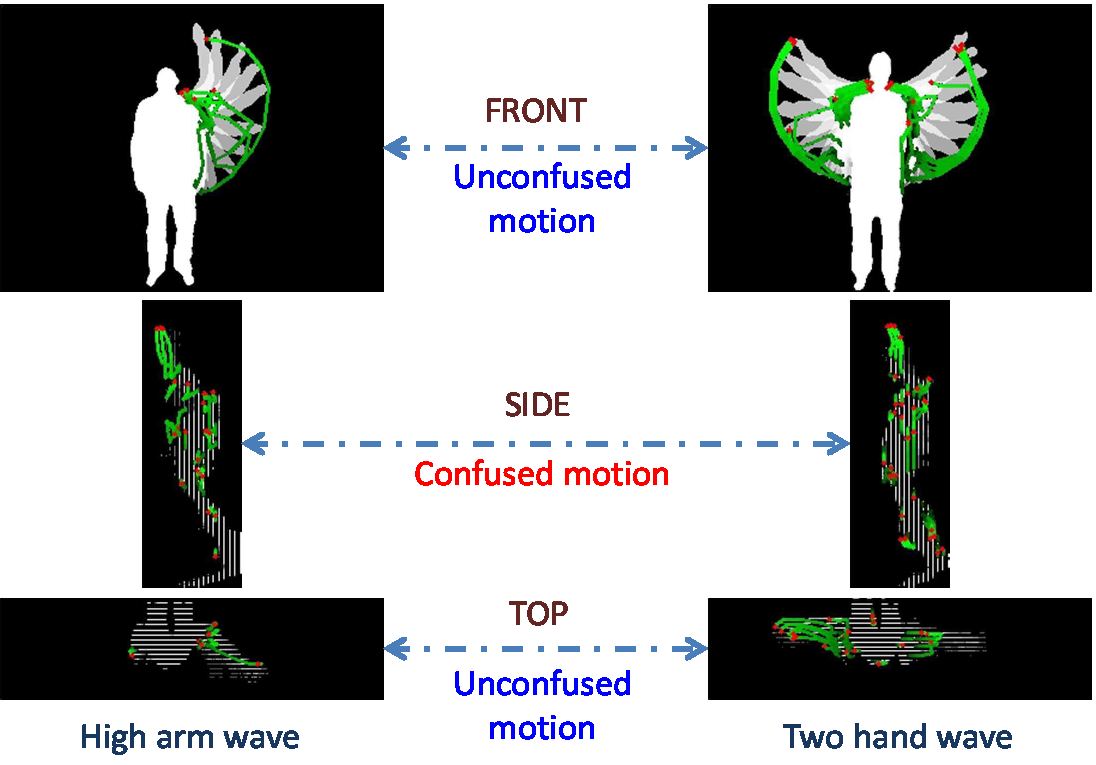
\includegraphics[width=\columnwidth]{Figures/Figure_TheRoleOfViews.pdf}
	\caption{Illustration of two actions \textit{high arm wave} and \textit{two hand wave}. We easily discriminate the two actions from front view and top view. But it is confused to label actions under side view.}
	\label{Figure_TheRoleOfViews}
\end{figure}

\subsubsection{The Role of Views}

Figure \ref{lbl:Figure_EarlyFusion_AS123_MBH} shows the role of views to our approach.
Experimental results confirm that action representations from front achieve the best performances. Obviously, the front view is an indispensable component to merge information.
Therefore, for the rest, we perform experiments on view combinations with front view.
%The performance of combinations is reported in figure \ref{lbl:Figure_CombinationsFRONTSIDETOP}. 
%In this experiment, the recognition accuracies of combinations are calculated on each intensity representations and the fusion.

\begin{figure*}[ht]
	\centering
	\resizebox{\textwidth}{!}{
	\begin{tabular}{cccccc}
	
	        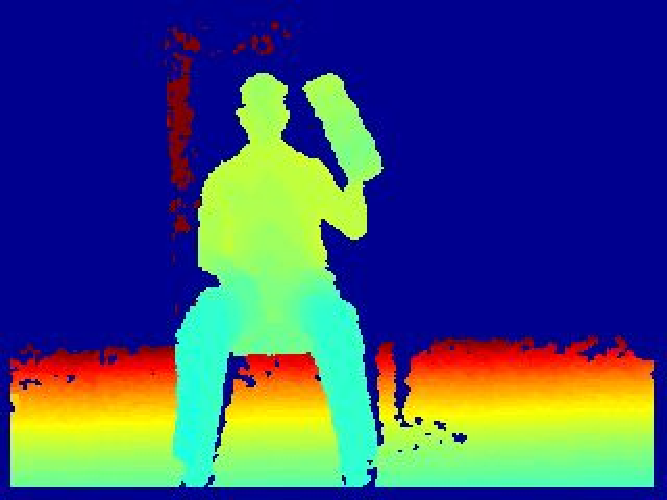
\includegraphics[width=0.15\textwidth]{Figures/Pair3D_pickup.pdf} &         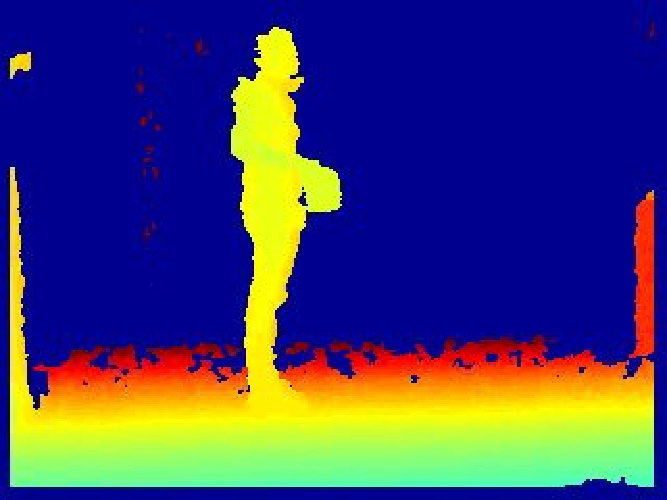
\includegraphics[width=0.15\textwidth]{Figures/Pair3D_lift.pdf} &         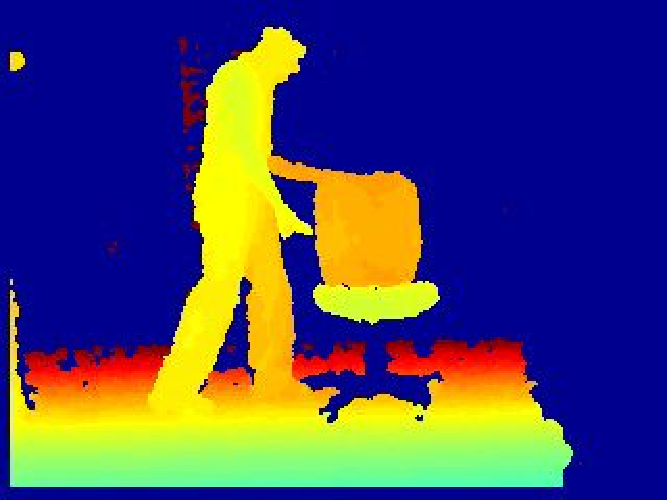
\includegraphics[width=0.15\textwidth]{Figures/Pair3D_push.pdf} &         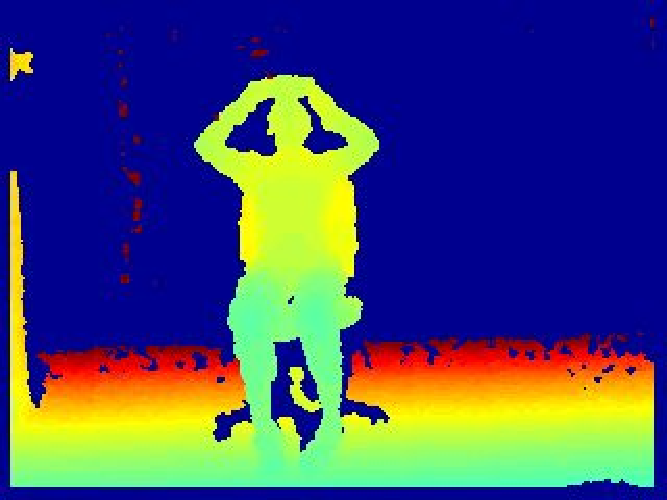
\includegraphics[width=0.15\textwidth]{Figures/Pair3D_wear.pdf} &         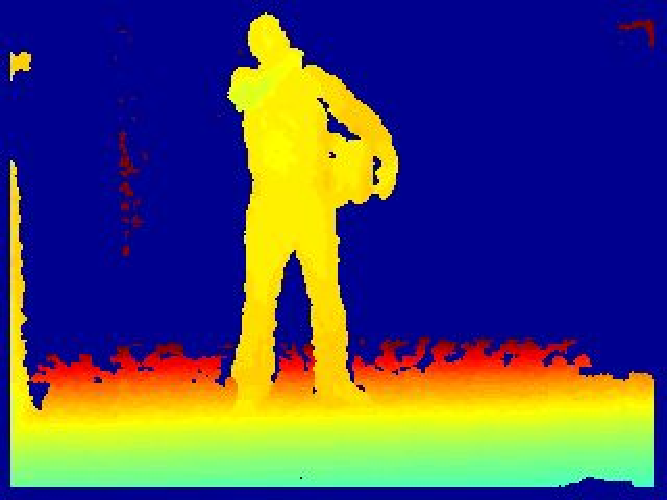
\includegraphics[width=0.15\textwidth]{Figures/Pair3D_putonabackpack.pdf} &         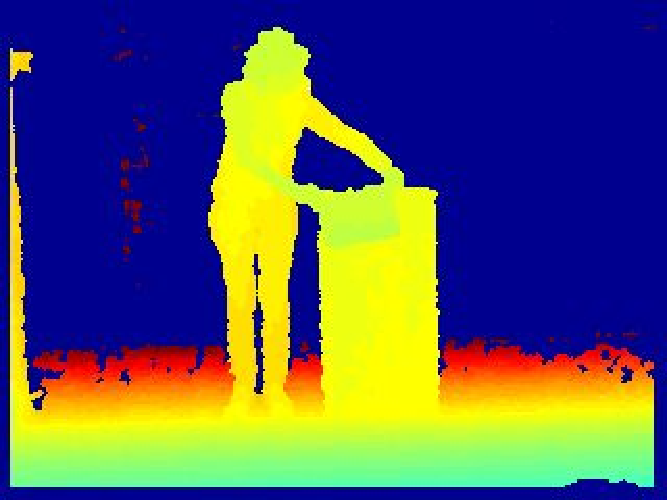
\includegraphics[width=0.15\textwidth]{Figures/Pair3D_stick.pdf} \\
	
	        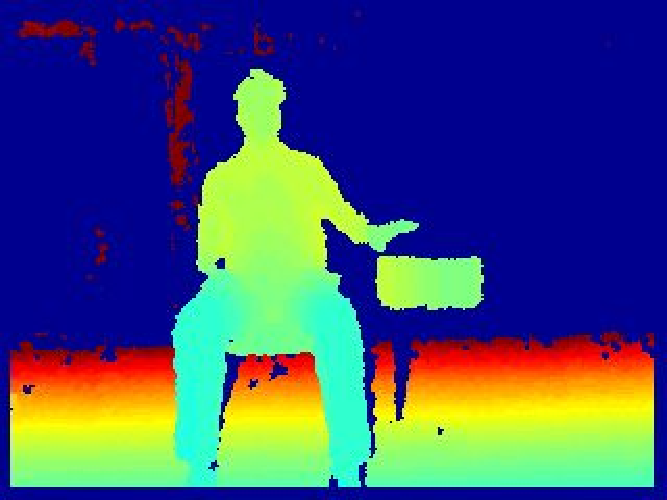
\includegraphics[width=0.15\textwidth]{Figures/Pair3D_putdown.pdf} &         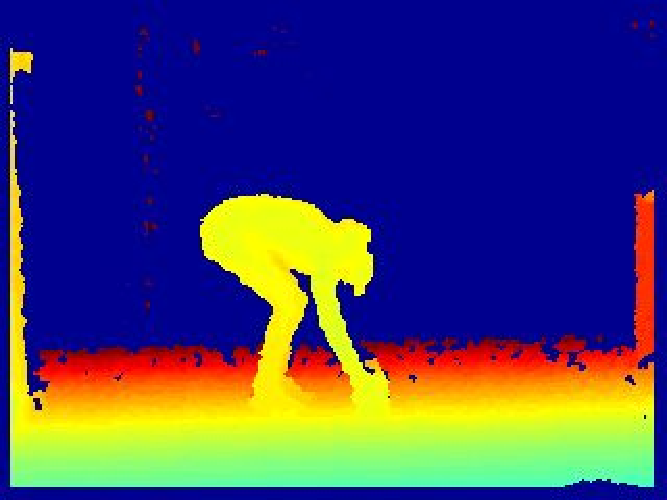
\includegraphics[width=0.15\textwidth]{Figures/Pair3D_place.pdf} &         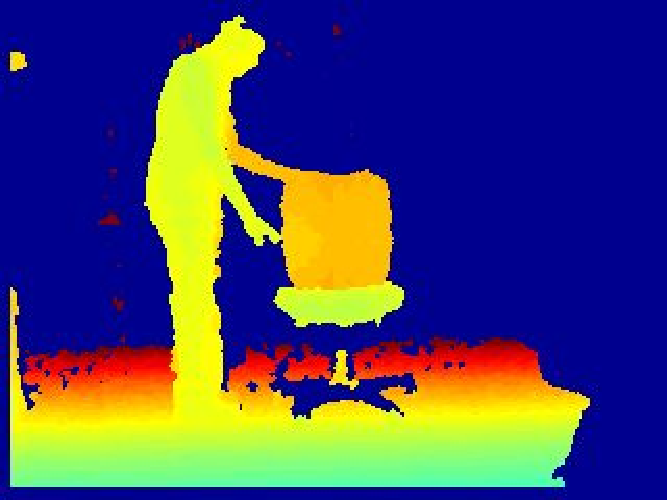
\includegraphics[width=0.15\textwidth]{Figures/Pair3D_pull.pdf} &         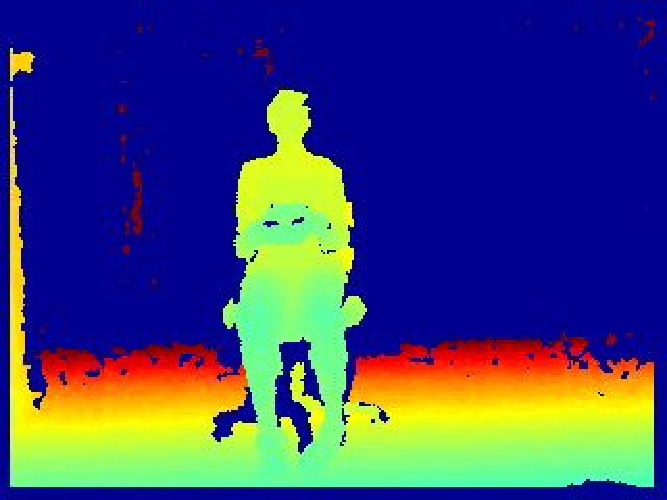
\includegraphics[width=0.15\textwidth]{Figures/Pair3D_takeoff.pdf} &         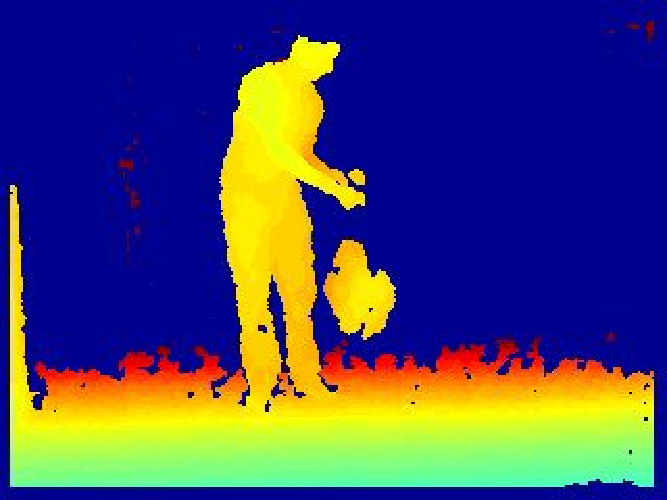
\includegraphics[width=0.15\textwidth]{Figures/Pair3D_takeoffabackpack.pdf} &         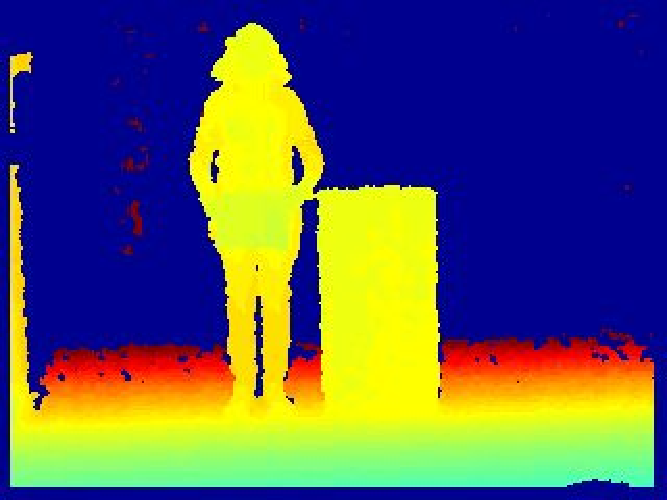
\includegraphics[width=0.15\textwidth]{Figures/Pair3D_remove.pdf} \\
	
	        Pick up/Put down &         Lift/Place &         Push/Pull &         Wear/Take off &         Put on/Take off &         Stick/Remove \\
	        
	        a box &         a box &         a chair &         a hat &         a backpack &         a poster \\
	
	\end{tabular}
	}
	\caption{Example frames for six pairs from 3D Action Pairs dataset \cite{oreifej2013hon4d}. Each column shows two frames from a pair of actions. Note that, for example in the first column, both actions: \textit{Pick up a box} and \textit{Put down a box} have similar motion information and shape cues; however, they are performed in different spatio-temporal order.}
	\label{Figure_ExampleFrames_3DActionPairs}
\end{figure*}

In order to conduct the experiments, we create additional combinations: front and side, front and top.
Figure \ref{Figure_CombinationsFRONTSIDETOP} shows the performance of the view combinations.
Interestingly, the achieved performance (96.95\%) from the combination of front and top beats the performance based on combining all the three views (96.67\%) as well as the combination of front and side (93.94\%), in terms of average accuracy.
In addition, based on experimental results, as described in figure \ref{Figure_CombinationsFRONTSIDETOP}, compensating information indicates two interesting points.

\begin{itemize}
	\item Firstly, compensating information from various views can cause unexpected risks, due to erroneous information from certain views.
	Indeed, consider two actions: \textit{high arm wave} and \textit{two hand wave}, although both contain ``wave arm'' movement, we easily recognize them from front and top views due to number of performed movements.
	However, if we observe the two actions from side view, a half of body is hidden by the rest (see figure \ref{Figure_TheRoleOfViews}).
	Therefore we confuse movements performed on the two actions.
	In this case, merging information from side view into the combination of front and top views causes to decrease the performance of the recognition system.
	
	\item Secondly, the experimental results have provided a good choice to decrease computational cost but still ensures a convincing performance.
	Looking at figure \ref{Figure_CombinationsFRONTSIDETOP}, we can see that the performances of two combinations, i.e. (front \& top) and (front \& side \& top), are comparable.
	In some cases, such as in action subsets 2, 3 and average, combination of front and top provide better performances.
	Obviously, if we eliminate unnecessary views, we can improve the efficiency of our system but still achieve competitive results.
\end{itemize}

These interesting points can lead to looking for optimal solution of combining views.
This is a promising challenge to overcome and build an effective and efficient recognition system.

\subsubsection{Comparison with the state-of-the-art}
Table \ref{lbl:Table_MBHvsSoAonFront} shows evaluation results of our proposed approach and the state-of-the-art approaches in terms of average accuracy on three action subsets from MSR Action 3D dataset (seeing table \ref{lbl:3ActionSubsets}).
The compared approaches are based on various feature representations, such as silhouette features \cite{li2010action, yang2012recognizing}, skeletal joint features like \cite{yang2012eigenjoints, wang2012mining}, local occupancy patterns \cite{wang2012robust, vieira2012stop}, normal orientation features \cite{oreifej2013hon4d} and cuboid similarity features \cite{xia2013spatio}.
Under the same setting (i.e cross subject test), the result table indicates that our approach beats all of them.

\begin{figure}[h]
	\centering
	\resizebox{\columnwidth}{!}{
		% Table generated by Excel2LaTeX from sheet 'Sheet3'
		\begin{tabular}{cccc}
			
			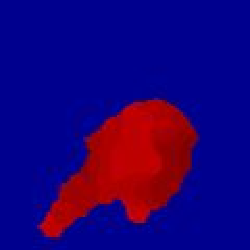
\includegraphics[width=0.22\columnwidth]{Figures/MSRGesture3D_bathroom.pdf} &          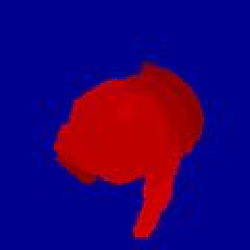
\includegraphics[width=0.22\columnwidth]{Figures/MSRGesture3D_blue.pdf} &          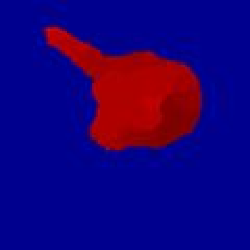
\includegraphics[width=0.22\columnwidth]{Figures/MSRGesture3D_finish.pdf} &          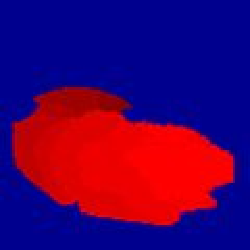
\includegraphics[width=0.22\columnwidth]{Figures/MSRGesture3D_green.pdf} \\
			
			1. Bathroom &          2. Blue &          3. Finish &          4. Green \\
			
			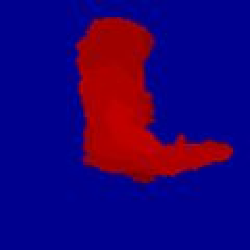
\includegraphics[width=0.22\columnwidth]{Figures/MSRGesture3D_hungry.pdf} &          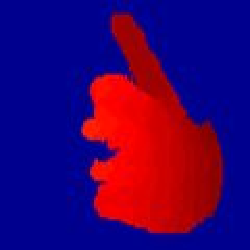
\includegraphics[width=0.22\columnwidth]{Figures/MSRGesture3D_milk.pdf} &          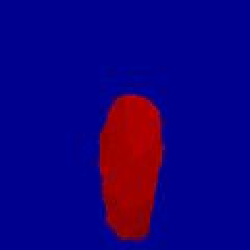
\includegraphics[width=0.22\columnwidth]{Figures/MSRGesture3D_past.pdf} &          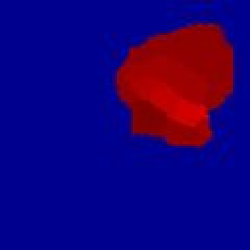
\includegraphics[width=0.22\columnwidth]{Figures/MSRGesture3D_pig.pdf} \\
			
			5. Hungry &          6. Milk &          7. Past &          8. Pig \\
			
			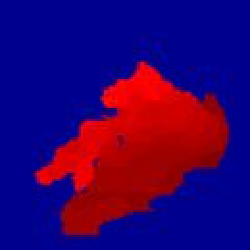
\includegraphics[width=0.22\columnwidth]{Figures/MSRGesture3D_store.pdf} &          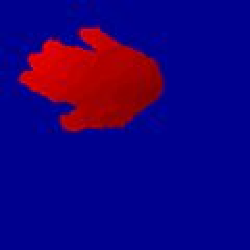
\includegraphics[width=0.22\columnwidth]{Figures/MSRGesture3D_where.pdf} &          \includegraphics[width=0.22\columnwidth]{Figures/MSRGesture3D_j.pdf} &          \includegraphics[width=0.22\columnwidth]{Figures/MSRGesture3D_z.pdf} \\
			
			9. Store &          10. Where &          11. J &          12. Z \\
			
		\end{tabular}  
		
	}
	\caption{Example frames for hand gestures from MSR Gesture 3D dataset \cite{wang2012robust}.}
	\label{Figure_ExampleFrames_MSRGesture3D}
\end{figure}

\subsection{MSR Gesture 3D Dataset}

The Gesture3D dataset \cite{wang2012robust} is a hand gesture dataset of depth sequences captured by a depth camera.
This dataset contains a set of gesture defined by American Sign Language (ASL).
In the dataset, there are 12 gestures as described in figure \ref{Figure_ExampleFrames_MSRGesture3D}.
There are ten subjects, each performs each gesture two or three times.
In total, the dataset contains 333 depth sequences.
The main challenge in the dataset is self-occlusion issue.
We follow the experimental settings in \cite{wang2012robust} (i.e. the leave-one-subject-out cross-validation) to evaluate our approach.
We obtain the accuracies described in table \ref{Table_MSRGesture3D_SoA}, where our approach outperforms all previous approaches.

\begin{table}[h]
	% Table generated by Excel2LaTeX from sheet 'Sheet3'
	\begin{tabular}{c|c}	
		    \bf Method & \bf Accuracy (\%) \\
		\hline
		X.Yang et al. \cite{yang2012recognizing}&       89.2 \\
		
		J.Wang et al. \cite{wang2012robust}&       88.5 \\
		
		O.Oreifej \& Z.Liu \cite{oreifej2013hon4d}&      92.45 \\
		\hline
		Ours (FRONT+SIDE) &      93.22 \\
		
		Ours (FRONT+TOP) &      92.66 \\
		
		\bf Ours (FRONT+SIDE+TOP) &      \bf 94.35 \\
	
	\end{tabular}  
	
	\caption{The performance of our approach on MSR Gesture 3D dataset, compared to previous approaches}
	\label{Table_MSRGesture3D_SoA}
\end{table}

\begin{table*}[ht]
	\centering
	\resizebox{\textwidth}{!}{
		% Table generated by Excel2LaTeX from sheet 'MBHHOGHOF'
		\begin{tabular}{c|c|c|c|c|c|c|c|c|c|}
			\hhline{~---------}
		           & \multicolumn{3}{c|}{MSR Action 3D} & \multicolumn{3}{c|}{MSR Gesture 3D} & \multicolumn{3}{c|}{3D Action Pairs} \\
		           
			\hhline{----------}
		\multicolumn{1}{|c|}{Combination} &  {\bf MBH} &  {\bf HOG} &  {\bf HOF} &  {\bf MBH} &  {\bf HOG} &  {\bf HOF} &  {\bf MBH} &  {\bf HOG} &  {\bf HOF} \\
		\hline
		\multicolumn{1}{|c|}{\bf FRONT+SIDE} &     93.94  &     93.01  &     91.82  &     93.22  &     {\bf 92.09}  &     89.83  &     92.22  &     82.78  &     92.22  \\
		\hline
		\multicolumn{1}{|c|}{\bf FRONT+TOP} &     {\bf 96.95}  &     92.14  &     {\bf 92.70}  &     92.66  &     90.40  &     88.14  &     {\bf 99.44}  &     {\bf 90.00}  &     {\bf 93.89}  \\
		\hline
		\multicolumn{1}{|c|}{\bf FRONT+SIDE+TOP} &     96.67  &     {\bf 94.53}  &     92.42  &     {\bf 94.35}  &     91.53  &     {\bf 92.09}  &     92.78  &     88.89  &     91.67  \\
		\hline
		\end{tabular}  
	}
	\caption{The performance of descriptors (MBH, HOG, and HOF) on MSR Action 3D dataset, MSR Gesture 3D datset, and 3D Action Pairs dataset. Evaluation criterion is average recognition accuracy; higher score means better performance.}
	\label{Table_MBHHOGHOF}
\end{table*}

\subsection{3D Action Pairs Dataset}

The 3D Action Pairs dataset \cite{oreifej2013hon4d} is a new type of action dataset.
The dataset contains pairs of actions, such that within each pair the motion and the shape cues are similar, but their correlations vary.
It is useful to evaluate how well the approaches capture the prominent cues jointly in depth sequences.
There are six pairs of actions, see figure \ref{Figure_ExampleFrames_3DActionPairs}.
Each action is performed three times by ten subjects, where the first five subjects are used for testing, and the rest for training.

\begin{table}[h]
	% Table generated by Excel2LaTeX from sheet 'Sheet3'
	\begin{tabular}{c|c}	
		\bf Method & \bf Accuracy (\%) \\
		\hline
		O.Oreifej \& Z.Liu \cite{oreifej2013hon4d}&      96.67 \\
		\hline
		Ours (FRONT+SIDE) &      92.22 \\
		
		\bf Ours (FRONT+TOP) &      \bf 99.44 \\
		
		Ours (FRONT+SIDE+TOP) &      92.78 \\
		
	\end{tabular}  
	
	\caption{The performance of our approach on 3D Action Pairs dataset, compared to the state-of-the-art approach.}
	\label{Table_3DActionPairs_SoA}
\end{table}

We compare our performance in this dataset with the HON4D approach \cite{oreifej2013hon4d}, which is the state-of-the-art performance until current time.
We summarize results in table \ref{Table_3DActionPairs_SoA}, and demonstrate the confusion tables in table \ref{Table_ConfusionMatrices_3DActionPairs}.
It is clear that our approach significantly outperforms the state-of-the-art approach for suffering from confusion appeared within action pairs.

\begin{table}[h]
	\centering
	\subfloat[O.Oreifej \& Z.Liu \cite{oreifej2013hon4d}]{
	\resizebox{\columnwidth}{!}{
		% Table generated by Excel2LaTeX from sheet 'ConfusionMatrix_3DActionPairs'
		\begin{tabular}{c|c|c|c|c|c|c|c|c|c|c|c|c|}
			\multicolumn{1}{c}{~} &  \multicolumn{1}{c}{\bf a01} &  \multicolumn{1}{c}{\bf a02} &  \multicolumn{1}{c}{\bf a03} &  \multicolumn{1}{c}{\bf a04} &  \multicolumn{1}{c}{\bf a05} &  \multicolumn{1}{c}{\bf a06} &  \multicolumn{1}{c}{\bf a07} &  \multicolumn{1}{c}{\bf a08} &  \multicolumn{1}{c}{\bf a09} &  \multicolumn{1}{c}{\bf a10} &  \multicolumn{1}{c}{\bf a11} &  \multicolumn{1}{c}{\bf a12} \\
			
			\hhline{~------------}
		 {\bf a01} &     \color{white}{\bf 1.0}\cellcolor[gray]{.0}  &          0 &          0 &          0 &          0 &          0 &          0 &          0  &          0 &          0 &          0 &          0 \\
			\hhline{~------------}
		 {\bf a02} &          0 &       \color{white}{\bf 1.0}\cellcolor[gray]{.0}  &          0 &          0 &          0 &          0 &          0 &          0 &          0 &          0 &          0 &          0 \\
			\hhline{~------------}
		 {\bf a03} &          0 &          0 &       \color{white}{\bf 0.80}\cellcolor[gray]{.2}  &          0 &          0 &          0 &          0 &          0 &          {\bf 0.133}\cellcolor[gray]{.8} &          {\bf 0.067}\cellcolor[gray]{.9} &          0 &          0 \\
			\hhline{~------------}
		 {\bf a04} &          0 &          0 &          0 &       \color{white}{\bf 0.933}\cellcolor[gray]{.1}  &          0 &          0 &          0 &          0 &          0 &          {\bf 0.067}\cellcolor[gray]{.9} &          0 &          0 \\
			\hhline{~------------}
		 {\bf a05} &          0 &          0 &          0 &          0 &       \color{white}{\bf 1.0}\cellcolor[gray]{.0}  &          0 &          0 &          0 &          0 &          0 &          0 &          0 \\
			\hhline{~------------}
		 {\bf a06} &          0 &          0 &          0 &          0 &          0 &       \color{white}{\bf 1.0}\cellcolor[gray]{.0}  &          0 &          0 &          0 &          0 &          0 &          0 \\
			\hhline{~------------}
		 {\bf a07} &          0 &          0 &          0 &          0 &          0 &          0 &       \color{white}{\bf 1.0}\cellcolor[gray]{.0}  &          0 &          0 &          0 &          0 &          0 \\
			\hhline{~------------}
		 {\bf a08} &          0 &          0 &          0 &          0 &          0 &          0 &          0 &       \color{white}{\bf 1.0}\cellcolor[gray]{.0}  &          0 &          0 &          0 &          0 \\
			\hhline{~------------}
		 {\bf a09} &          0 &          0 &          0 &          0 &          0 &          0 &          0 &          0 &       \color{white}{\bf 1.0}\cellcolor[gray]{.0}  &          0 &          0 &          0 \\
			\hhline{~------------}
		 {\bf a10} &          0 &          0 &          0 &          0 &          0 &          0 &          0 &          0 &          0 &       \color{white}{\bf 1.0}\cellcolor[gray]{.0}  &          0 &          0 \\
			\hhline{~------------}
		 {\bf a11} &          0 &          0 &          0 &          0 &          0 &          0 &          0 &          0 &          0 &          0 &       \color{white}{\bf 1.0}\cellcolor[gray]{.0}  &          0 \\
			\hhline{~------------}
		 {\bf a12} &          0 &          0 &          0 &          0 &          0 &          0 &          0 &          0 &          0 &          0 &          {\bf 0.133}\cellcolor[gray]{.8} &       \color{white}{\bf 0.867}\cellcolor[gray]{.2}  \\
			\hhline{~------------}
		\end{tabular} 
	}
	}
	
	\subfloat[Ours (FRONT+TOP)]{
		\resizebox{\columnwidth}{!}{
			% Table generated by Excel2LaTeX from sheet 'ConfusionMatrix_3DActionPairs'
			\begin{tabular}{c|c|c|c|c|c|c|c|c|c|c|c|c|}
				\multicolumn{1}{c}{~} &  \multicolumn{1}{c}{\bf a01} &  \multicolumn{1}{c}{\bf a02} &  \multicolumn{1}{c}{\bf a03} &  \multicolumn{1}{c}{\bf a04} &  \multicolumn{1}{c}{\bf a05} &  \multicolumn{1}{c}{\bf a06} &  \multicolumn{1}{c}{\bf a07} &  \multicolumn{1}{c}{\bf a08} &  \multicolumn{1}{c}{\bf a09} &  \multicolumn{1}{c}{\bf a10} &  \multicolumn{1}{c}{\bf a11} &  \multicolumn{1}{c}{\bf a12} \\
				
				\hhline{~------------}
			 {\bf a01} &     \color{white}{\bf 0.933}\cellcolor[gray]{.1}  &          0 &          0 &          0 &          0 &          0 &          0 &     {\bf 0.067}\cellcolor[gray]{.9}  &          0 &          0 &          0 &          0 \\
				\hhline{~------------}
			 {\bf a02} &          0 &       \color{white}{\bf 1.0}\cellcolor[gray]{.0}  &          0 &          0 &          0 &          0 &          0 &          0 &          0 &          0 &          0 &          0 \\
				\hhline{~------------}
			 {\bf a03} &          0 &          0 &       \color{white}{\bf 1.0}\cellcolor[gray]{.0}  &          0 &          0 &          0 &          0 &          0 &          0 &          0 &          0 &          0 \\
				\hhline{~------------}
			 {\bf a04} &          0 &          0 &          0 &       \color{white}{\bf 1.0}\cellcolor[gray]{.0}  &          0 &          0 &          0 &          0 &          0 &          0 &          0 &          0 \\
				\hhline{~------------}
			 {\bf a05} &          0 &          0 &          0 &          0 &       \color{white}{\bf 1.0}\cellcolor[gray]{.0}  &          0 &          0 &          0 &          0 &          0 &          0 &          0 \\
				\hhline{~------------}
			 {\bf a06} &          0 &          0 &          0 &          0 &          0 &       \color{white}{\bf 1.0}\cellcolor[gray]{.0}  &          0 &          0 &          0 &          0 &          0 &          0 \\
				\hhline{~------------}
			 {\bf a07} &          0 &          0 &          0 &          0 &          0 &          0 &       \color{white}{\bf 1.0}\cellcolor[gray]{.0}  &          0 &          0 &          0 &          0 &          0 \\
				\hhline{~------------}
			 {\bf a08} &          0 &          0 &          0 &          0 &          0 &          0 &          0 &       \color{white}{\bf 1.0}\cellcolor[gray]{.0}  &          0 &          0 &          0 &          0 \\
				\hhline{~------------}
			 {\bf a09} &          0 &          0 &          0 &          0 &          0 &          0 &          0 &          0 &       \color{white}{\bf 1.0}\cellcolor[gray]{.0}  &          0 &          0 &          0 \\
				\hhline{~------------}
			 {\bf a10} &          0 &          0 &          0 &          0 &          0 &          0 &          0 &          0 &          0 &       \color{white}{\bf 1.0}\cellcolor[gray]{.0}  &          0 &          0 \\
				\hhline{~------------}
			 {\bf a11} &          0 &          0 &          0 &          0 &          0 &          0 &          0 &          0 &          0 &          0 &       \color{white}{\bf 1.0}\cellcolor[gray]{.0}  &          0 \\
				\hhline{~------------}
			 {\bf a12} &          0 &          0 &          0 &          0 &          0 &          0 &          0 &          0 &          0 &          0 &          0 &       \color{white}{\bf 1.0}\cellcolor[gray]{.0}  \\
				\hhline{~------------}
			\end{tabular} 
		}
		}
	\caption{The confusion tables for 3D Action Pairs dataset.}
	\label{Table_ConfusionMatrices_3DActionPairs}
\end{table}

\section{Discussion}
\label{Section_Discussion}

%\subsection{The Impact of Our Method on Descriptors}
\paragraph{The Impact of Our Method on Descriptors}

For intensity data, according to \cite{wang2011densetraj} MBH is the best feature descriptor for dense trajectories. Therefore, in previous experiments, we only use MBH descriptor to represent motion information. Due to the difference between depth data and intensity data, how our approach has influenced other trajectory-aligned descriptors (i.e. HOG, HOF). In this part, we conduct similar experiments on these descriptors to answer this issue.

We report the average recognition accuracies on the three descriptors and on the combinations of the three views: front, side, and top. Table \ref{Table_MBHHOGHOF} shows interesting results.
Firstly, experimental results verify that the MBH descriptor is still the best trajectory-aligned descriptor in comparison with the HOG, HOF descriptors on the experimental datasets.
Secondly, although the HOG, HOF descriptors are not the best, their performance is comparable to the state-of-the-art approaches, as mentioned in section \ref{Section_Experiments}.
In addition, lower-cost descriptors like HOG, HOF have more benefits for decreasing computational cost in processes, such as feature extraction and video representation (using the BoW model).
These advantages provide a promising way for building effective and efficient systems.

\section{Conclusions}
\label{Section_Conclusions}

We proposed a trajectory-based approach to effectively exploit discriminative motion patterns for human action recognition using depth sequences in this work.
The motion patterns based on trajectories jointly encodes local motion and appearance cues.
In order to deal with confused actions due to similar movements, compensating information from different observation views is proposed.
In addition, we also analyze the role of views in compensating information.
We have evaluated our proposed approach extensively on three challenging benchmark datasets and shown that it significantly outperforms the state-of-the-art.

Our trajectory-based approach with compensating information from separate motion representations shows promising results.
This opens a more general approach to optimize the view selection for combinations.
This also suggests the importance of discriminative motion patterns for human action recognition on depth sequences.
Therefore, exploiting depth-based motion trajectories can be beneficial for action recognition systems using depth cameras.
This is also an interesting idea for our future work.

\section*{References}

\bibliographystyle{splncs}
\bibliography{JournalPaper_Ref}
\biboptions{sort&compress}

\end{document}